\documentclass[12pt]{article}
\usepackage[utf8]{inputenc}
\usepackage[T2A]{fontenc}
\usepackage[russian]{babel}
\usepackage{amsmath}
\usepackage{amssymb}
\usepackage{dsfont}
\usepackage[dvipsnames]{xcolor}
\usepackage{setspace}
\usepackage{multirow}
\usepackage[a4paper, outer=1.5cm, inner=1.5cm, top=1cm, bottom=1cm]{geometry}
\usepackage{graphicx}
\usepackage{skull}
\usepackage{wasysym}
\usepackage{float}
\graphicspath{{.images/}}
\usepackage{hyperref}
\hypersetup{colorlinks=true, linkcolor=blue, filecolor=magenta, urlcolor=cyan}
\usepackage[firstpage]{draftwatermark}
\SetWatermarkText{
    $\qquad\qquad\qquad\qquad\qquad$\parbox{7cm}{\begin{center}
    
\includegraphics[width = 0.08\textwidth]{lion-logo.png}\bigskip\\~\bigskip\\~\vspace{-24mm}\\~\end{center}}
}
\SetWatermarkAngle{0}
\SetWatermarkScale{1.5}
\usepackage{etoolbox}

\newtoggle{ifsolved}
\newtoggle{needhelp}
\newcounter{num}
\setcounter{num}{1}

\newcommand{\newnum}{\par\textbf{\textnumero\arabic{num}}\stepcounter{num}}
\newcommand{\sol}{\vspace{3mm}\par\textbf{Решение: }}
\newcommand{\ans}{\vspace{3mm}\par\textbf{Ответ: }}
\newcommand{\hint}{\vspace{3mm}\par\textbf{Подсказка: }}
\newcommand{\mode}[1]{
\ifstrequal{#1}{0}{\togglefalse{ifsolved}\togglefalse{needhelp}}{\ifstrequal{#1}{1}{\togglefalse{ifsolved}\toggletrue{needhelp}}{\ifstrequal{#1}{2}{\toggletrue{ifsolved}\togglefalse{needhelp}}{\toggletrue{ifsolved}\toggletrue{needhelp}}}}} %if 0 - if 1 - if 2 - else
%\newenvironment{problem}[8]{%#1, #2, #3
%\parbox{\linewidth}{\vspace{4mm}\ifstrequal{#4}{(лёгкая)}{\newnum\textbf{.}}{\newnum\textbf{*.} } \\ #5}
%\iftoggle{ifsolved}{\sol #6}{}
%\iftoggle{ifsolved}{\ans #7}{}
%\iftoggle{needhelp}{\hint #8}{}}

\newenvironment{problem}[8]{%#1, #2, #3
\parbox{\linewidth}{\vspace{5mm}\ifstrequal{#4}{(лёгкая)}{\newnum\textbf{.}}{\newnum\textbf{*.} } \\ #5}
\iftoggle{ifsolved}{\sol #6}{}

\iftoggle{ifsolved}{\parbox{\linewidth}{\ans #7}}{}
\iftoggle{needhelp}{\parbox{\linewidth}{\hint #8}}{}}

\newenvironment{mylist} %custom list
{ \begin{itemize}
    \setlength{\itemsep}{0pt}
    \setlength{\parskip}{0pt}
    \setlength{\parsep}{0pt}     }
{ \end{itemize}                  }

\newenvironment{homeass}[1]{\vspace*{-1.5cm}
\iftoggle{ifsolved}{
    \section*{\center{Решение домашнего задания к #1.}}
}{
    \section*{\center{\textcolor{Sepia}{Домашнее задание к #1}}}
} \vspace{7mm}\large}

\parindent=0pt
\pagestyle{empty}
%$\!$[\arabic{class}.\arabic{num}]
%\ifnumcomp{\value{counter}}{>}{1}{true}{false}
%\definecolor{Gray}{gray}{0.9}
%\definecolor{mypink}{RGB}{219, 48, 122}
%\newcolumntype{g}{>{\columncolor{Gray}}p{2.8cm}}

\begin{document}
\large
\mode{7}
%0 for problems without hints
%1 for problems + hints
%2 for problems + solutions + answers
%else: show all

{\centering\section*{СПИСОК ЗАДАЧ}}

{\centering\subsection*{\smallskip\\\textcolor{green}{\textbf{Полезные вещи, которые можно и нужно копипастить:}}}}

\subsection*{\textcolor{Emerald}{\textbf{Полезные шпаргалки по LaTeXу:}}}

\textbf{Пример вставки рисунка:}

\begin{minipage}{\linewidth}
    \begin{minipage}{0.54\linewidth}
    см. рисунок справа\\
    Текст к собственно пикче, примерно всегда это либо развёрнутое описание, либо большая часть решения задачи --- стремимся экономить пространство, если это можно сделать.
    \end{minipage}
    \hspace{0.05\linewidth}
    \begin{minipage}{0.4\linewidth}
    \begin{figure}[H] 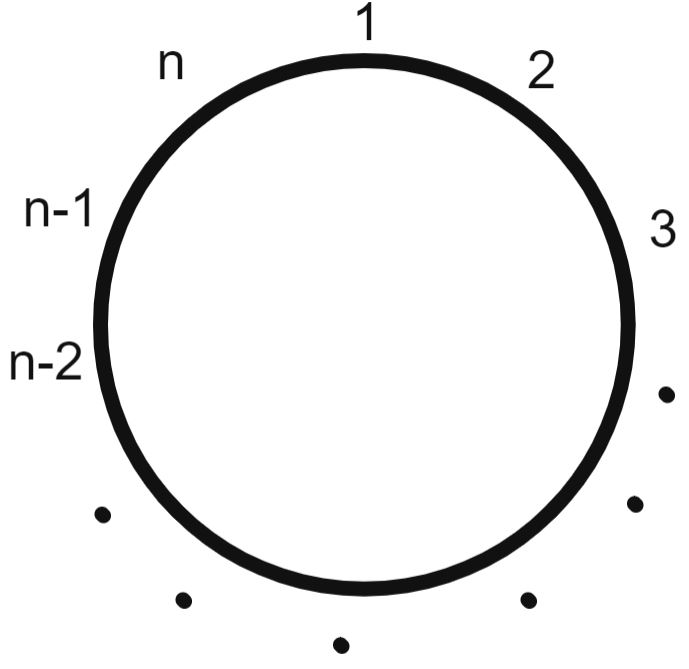
\includegraphics[width=\linewidth]{sol3} %тут поменять имя пикчи
    \end{figure}
    \end{minipage}
\end{minipage}

\textbf{Дефолтные математические знаки и символы:}\\
$\geqslant$,
$\leqslant$,
$a^{b}$,
$x_{i}$,
$\sqrt{a}$,
$\frac{a}{b}$,
$\displaystyle \frac{a}{b}$,
$\cdot$
$\;\Rightarrow\;$,
$\;\Leftrightarrow\;$,
$1{,}2$.
О промежутках:
$a\!b$,
$a\,b$,
$a\:b$,
$a\;b$,
$a\quad b$.

\textbf{Стандартные система и совокупность уравнений / неравенств:}\\
$\left\{
\begin{aligned}
f(x) &= 0 \\
g(x) &= 1
\end{aligned}\right.$

$\left[\begin{aligned}
&\left\{\begin{aligned}
f(x) &\geqslant a \\
g(x) &= b
\end{aligned}\right.\\
&\left\{\begin{aligned}
f(x) &< a \\
g(x) &= -b
\end{aligned}\right.
\end{aligned}\right.$

\subsection*{\textcolor{Emerald}{\textbf{Не математическое, но полезное:}}}
% комментарий в любом месте документа, который нигде не будет видно. Можно использовать для написания заметок-вопросов по задачам
\textbf{Пример таблицы:}

\begin{tabular}{|c|c|c|}
\hline
    $a$ & $b$ & текст
\\\hline
    $c$ & $d$ & мораль
\\\hline
\end{tabular}\\

\textbf{Отступы:} между\smallskip\\ строками\medskip\\ \textbf{Тире} --- это три дефиса.\\
\textbf{Списки:}
\begin{mylist}
\item [$\bullet$] это был пункт а
\item [2)] а это уже пункт номер 2 с изменённым заголовком
\end{mylist}

\subsection*{\textcolor{Emerald}{\textbf{Всё, неупомянутое выше (или если просто что-то не так):}}}
\begin{mylist}
\item [$\bullet$] Решение отдельных вопросов касательно ТеХа нужно искать в \href{https://www.mccme.ru/free-books/llang/newllang.pdf}{Львовском}.

\item [$\bullet$] Найти произвольный символ, который нужен, можно в \href{http://detexify.kirelabs.org/classify.html}{Detexify}.

\item [$\bullet$] Если возникли сомнения при решении, ответ практически ко всем задачам можно проверить с помощью \href{https://www.wolframalpha.com/}{WolframAlpha}.

\item [$\bullet$] Если в задаче нужно создать картинку, то лучше пока отложить эту задачу. Все графики планируется централизованно нарисовать (или перерисовать) в геогебре.

\item [\textcolor{brown}{\textbf{!!}}] Важно ставить \textcolor{red}{\textbf{$\spadesuit$}}
(или просто red) в тело задачи в случае серьёзных вопросов к решению и какой-то вопиющей лажи.

\item [\textcolor{brown}{\textbf{!!}}] Важно ставить \textcolor{olive}{\textbf{$\spadesuit$}}
(или просто olive) в тело задачи в случае не самого удачного текста и кривых отступов.
\end{mylist}

\subsection*{\textcolor{Violet}{\textbf{Комментарии:}}}% а также невидимые комментарии - так можно оставлять заметки-вопросы прямо в задаче, чтобы потом было понятно, в чём вопрос.
\begin{mylist}
\item [$\skull$] Переставлять задачи местами --- очень плохая идея.

\item [$\smiley$] При двойном клике по тексту pdf справа происходит автоматический переход к этому месту в латех-коде, а для обратного перехода можно нажать стрелку вправо (висит сверху между pdf и латех-кодом).

\item [$\smiley$] Если есть размышления, дописывать red/olive к задаче или не дописывать, то лучше всё-таки дописать.

\item [$\skull$] Самое плохое, что можно сделать --- написать в любое поле из трёх (НаписанноеРешение/ВерныйОтвет/Подсказка) только половину того, что надо, никак это не отметить, и потом пойти дальше.\\ Нужно в этот момент писать red/olive в случайном месте задачи, чтобы потом вычислить это с помощью Ctrl+F по всему документу (и это то, что потом будет делаться долго и тщательно)
\end{mylist}

\newpage
\setcounter{num}{1232}

\hypertarget{9.3}{{\centering\section*{\bigskip\\\textcolor{Blue}{\hyperlink{start2}{\textcolor{Blue}{9.3}} Системы уравнений и неравенств с двумя неизвестными.}\vspace{-5mm}}}}

\begin{problem}{Уравнения с двумя неизвестными.}{9.3.1}{X}{(лёгкая)}
{Нарисовать на декартовой плоскости все точки, являющиеся решениями уравнения $(y - 3) \cdot (x + 2) = 0$. Осторожно~--- это НЕ функция!}
{НаписанноеРешение}
{ВерныйОтвет}{Подсказка}
\end{problem}

\begin{problem}{Неравенства с двумя переменными.}{9.3.2}{79I}{(лёгкая)}
{\vspace{-2mm}\\\parbox{0.53\linewidth}{Изобразить на координатной плоскости фигуру, точки которой являются решением системы неравенств, написанной справа.\medskip\\ Найти площадь этой фигуры.}
$\quad\left\{
\begin{aligned}
    \: x &> 0\\
    \: y &> 0\\
    \: y &< 16 - 2x\\
    \: y &< 9 - x\\
    \: 5y &< 25 - x
\end{aligned}\right.$}
{НаписанноеРешение}
{ВерныйОтвет}{Подсказка}
\end{problem}

\begin{problem}{Неравенства с двумя переменными.}{9.3.2}{9D}{*}
{Решить уравнение $(x - 3)(y + 2)(xy - 2x + 3)(xy + 3y - 4) = 0$. Нарисовать график этого уравнения и отметить те области, где данное выражение положительно.}
{НаписанноеРешение}
{ВерныйОтвет}{Подсказка}
\end{problem}

\begin{problem}{Системы уравнений и неравенств с двумя переменными.}{9.3.3}{9I}{(лёгкая)}
{Решить систему уравнений $\;\left\{
\begin{aligned}
    \: (x - 4)(y + 3) &= 0\\
    \: 4y - 3x =&\; 12.
\end{aligned}\right.$}
{НаписанноеРешение}
{ВерныйОтвет}{Подсказка}
\end{problem}

\begin{problem}{Системы уравнений и неравенств с двумя переменными.}{9.3.3}{9D}{(лёгкая)}
{Составить уравнение окружности, проходящей через точки $A(-2; 1)$, $B(9; 3)$, $C(1; 7)$.

}
{НаписанноеРешение}
{ВерныйОтвет}{Подсказка}
\end{problem}

\begin{problem}{Системы уравнений и неравенств с двумя переменными.}{9.3.3}{9D}{(лёгкая)}
{\vspace{-2mm}\\\parbox{0.7\linewidth}{Решить систему линейных неравенств при $x > 0$, $y > 0$:\medskip\\Найти площадь получившейся фигуры.}
$\quad\left\{\begin{aligned}
    4y + 3x &\leqslant 24\\
    2y + 2x &\leqslant 13\\
    2y + 5x &\leqslant 25
\end{aligned}\right.$\\ }
{НаписанноеРешение}
{ВерныйОтвет}{Подсказка}
\end{problem}

\begin{problem}{Системы уравнений и неравенств с двумя переменными.}{9.3.3}{9D}{(лёгкая)}
{Решить систему неравенств:
$\quad\left\{\begin{aligned}
    a &< b + 1\\
    b &< a + 1\\
    ab &< 2
\end{aligned}\right.$}
{НаписанноеРешение}
{ВерныйОтвет}{Подсказка}
\end{problem}

\begin{problem}{Системы уравнений и неравенств с двумя переменными.}{9.3.3}{9I}{(лёгкая)}
{Решить систему: $\;\left\{
\begin{aligned}
    \: x^{2} + y^{2} &\leqslant 10\\
    \: xy &= 3
\end{aligned}\right.$\\
Нарисовать ГМТ точек, являющихся решениями этой системы.}
{НаписанноеРешение}
{ВерныйОтвет}{Подсказка}
\end{problem}

\begin{problem}{Системы уравнений и неравенств с двумя переменными.}{9.3.3}{9I}{(лёгкая)}
{Решить совокупность уравнений и неравенств:
$\;\left[\begin{aligned}
    \left\{
\begin{aligned}
    \: x^{2} + y^{2} &\leqslant 5\\
    \: xy =&\; 2
\end{aligned}\right.\\
\left\{
\begin{aligned}
    \: x^{2} + y^{2} &= 5\\
    \: xy \leqslant&\; 2
\end{aligned}\right.
\end{aligned}
\right.$\\
Нарисовать ГМТ точек, являющихся решениями этой системы.}
{НаписанноеРешение}
{ВерныйОтвет}{Подсказка}
\end{problem}

\begin{problem}{Системы уравнений и неравенств с двумя переменными.}{9.3.3}{9D}{(лёгкая)}
{Решить систему уравнений:
$\quad\left\{\begin{aligned}
    x^{2} + y^{2} &= 25\\
    3x - 4y &= 0
\end{aligned}\right.$}
{НаписанноеРешение}
{ВерныйОтвет}{Подсказка}
\end{problem}

\begin{problem}{Системы уравнений и неравенств с двумя переменными.}{9.3.3}{9D}{*}
{На координатной плоскости изобразить множество точек, удовлетворяющих неравенству $x^{2}y - 4y \leqslant 0$.}
{НаписанноеРешение}
{ВерныйОтвет}{Подсказка}
\end{problem}

\begin{problem}{Методы решения систем уравнений.}{9.3.4}{7A}{(лёгкая)}
{Решить систему уравнений: $\quad\left\{
\begin{aligned}
    \: 3x - y &= 2\\
    \: x^{2} - 4x &+ 8 = y
\end{aligned}\right.$}
{НаписанноеРешение}
{ВерныйОтвет}{Подсказка}
\end{problem}

\begin{problem}{Методы решения систем уравнений.}{9.3.4}{7A}{(лёгкая)}
{Решить систему уравнений: $\quad\left\{
\begin{aligned}
    \: |x^{2} - 4y^{2}| &= x^{2} - 4\\
    \: x^{2} = 4y^{2} &+ 5
\end{aligned}\right.$}
{НаписанноеРешение}
{ВерныйОтвет}{Подсказка}
\end{problem}

\begin{problem}{Методы решения систем уравнений.}{9.3.4}{7A}{(лёгкая)}
{Решить систему уравнений:
$\quad\left\{
\begin{aligned}
    \: x &+ 2y = 13\;\quad\\
    \: &xy = \, 15
\end{aligned}\right.$}
{НаписанноеРешение}
{ВерныйОтвет}{Подсказка}
\end{problem}

\begin{problem}{Методы решения систем уравнений.}{9.3.4}{7A}{(лёгкая)}
{Решить систему уравнений:
$\quad\left\{
\begin{aligned}
    \: 9x^{2} + 25y^{2} &= 5x + 30xy - 2y\;\quad\\
    \: 3x &= 5y + 2
\end{aligned}\right.$}
{НаписанноеРешение}
{ВерныйОтвет}{Подсказка}
\end{problem}

\begin{problem}{Методы решения систем уравнений.}{9.3.4}{7A}{(лёгкая)}
{Решить систему уравнений:
$\quad\left\{
\begin{aligned}
    \: x^{2} + y^{2} &- 2x - 3y = -1\;\quad\\
    \: x^{2} + y^{2} &= 10
\end{aligned}\right.$}
{НаписанноеРешение}
{ВерныйОтвет}{Подсказка}
\end{problem}

\begin{problem}{Методы решения систем уравнений.}{9.3.4}{7A}{(лёгкая)}
{Решить уравнение: $\,(x^{2} - 25)^{2} + (x^{2} + 3x - 10)^{2} = 0$.}
{НаписанноеРешение}
{ВерныйОтвет}{Подсказка}
\end{problem}

\begin{problem}{Методы решения систем уравнений.}{9.3.4}{7A}{(лёгкая)}
{Решить уравнение: $\,(x^{2} - 16)^{2} + (x^{2} + x - 12)^{2} = 0$.}
{НаписанноеРешение}
{ВерныйОтвет}{Подсказка}
\end{problem}

\begin{problem}{Методы решения систем уравнений.}{9.3.4}{9I}{(лёгкая)}
{Окружность $x^{2} + y^{2} = 10$ и прямая $y = 2x + 5$ пересекаются в точках $A$ и $B$.\\ Найти уравнение, которое задаёт прямую, являющуюся срединным\\ перпендикуляром к отрезку $AB$.}
{НаписанноеРешение}
{ВерныйОтвет}{Подсказка}
\end{problem}

\begin{problem}{Методы решения систем уравнений.}{9.3.4}{6K}{(лёгкая)}
{Из А в В и из В в А одновременно на рассвете вышли навстречу друг другу (по одной дороге) две старушки. Они встретились в полдень (12:00), но не остановились, а продолжили идти с теми же скоростями, и первая пришла в В в 4 часа дня (16:00), а вторая (в А) в девять часов вечера (21:00).\\
В котором часу был в этот день рассвет?}
{НаписанноеРешение}
{ВерныйОтвет}{Подсказка}
\end{problem}

\begin{problem}{Методы решения систем уравнений.}{9.3.4}{6S}{(лёгкая)}
{Очевидно, что верны уравнения $\quad\begin{aligned}
2 \text{ руб.} &= 200 \text{ коп.}\\
0{,}25 \text{ руб.} &= 25 \text{ коп.}
\end{aligned}\quad $\\
Однако, перемножив эти равенства, получим $0{,}5 \text{ руб.} = 5000 \text{ коп.}$ Где ошибка?

}
{НаписанноеРешение}
{ВерныйОтвет}{Подсказка}
\end{problem}

\begin{problem}{Методы решения систем уравнений.}{9.3.4}{6K \textcolor{olive}{\textbf{$\spadesuit$}}}{(лёгкая)}
{\vspace{-6mm}\\\begin{minipage}{\linewidth}
    \begin{minipage}{0.5\linewidth}

    На рисунке справа изображены $9$ прямоугольников, а также указаны площади трёх маленьких прямоугольников. Чему равна неизвестная площадь?

    \end{minipage}
    \hspace{0.05\linewidth}
    \begin{minipage}{0.44\linewidth}
        \begin{figure}[H]
        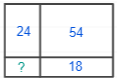
\includegraphics[width=\linewidth]{6K-23}
        \end{figure}
    \end{minipage}
\end{minipage}}
{НаписанноеРешение}
{ВерныйОтвет}{Подсказка}
\end{problem}

\begin{problem}{Методы решения систем уравнений.}{9.3.4}{9D}{(лёгкая)}
{Решить систему уравнений:
$\quad\left\{
\begin{aligned}
    \:\frac{1}{x} &= y + z\\
    \:\frac{1}{y} &= x + z\\
    \:\frac{1}{z} &= x + y
\end{aligned}\right.$}
{НаписанноеРешение}
{ВерныйОтвет}{Подсказка}
\end{problem}

\begin{problem}{Методы решения систем уравнений.}{9.3.4}{9D}{(лёгкая)}
{Решить систему уравнений:
$\quad\left\{
\begin{aligned}
    \: xy - t^{2} = 9\;\quad\\
    \: x^{2} + y^{2} + z^{2} = 18
\end{aligned}\right.$}
{НаписанноеРешение}
{ВерныйОтвет}{Подсказка}
\end{problem}

\begin{problem}{Методы решения систем уравнений.}{9.3.4}{9D кув *?}{(лёгкая)}
{Найти наименьшее значение $x^{2} + y^{2}$, если $x^{2} - y^{2} + 6x + 4y + 5 = 0$.}
{НаписанноеРешение}
{ВерныйОтвет}{Подсказка}
\end{problem}

\begin{problem}{Методы решения систем уравнений.}{9.3.4}{9D red скорее всего *}{(лёгкая)}
{Найти все положительные решения системы уравнений
$\quad\left\{
\begin{aligned}
    \: x_1 + x_2 &= x_3^{2}\\
    \: x_2 + x_3 &= x_4^{2}\\
    \: x_3 + x_4 &= x_5^{2}\\
    \: x_4 + x_5 &= x_1^{2}\\
    \: x_5 + x_1 &= x_2^{2}
\end{aligned}\right.$}
{НаписанноеРешение}
{ВерныйОтвет}{Подсказка}
\end{problem}

\begin{problem}{Методы решения систем уравнений.}{9.3.4}{9I}{(лёгкая)}
{Решить систему уравнений:
$\quad\left\{\begin{aligned}
    \frac{y}{x} + \frac{x}{y} &= \frac{13}{6}\\
    x + y &= 5
\end{aligned}\right.$}
{НаписанноеРешение}
{ВерныйОтвет}{Подсказка}
\end{problem}

\begin{problem}{Методы решения систем уравнений.}{9.3.4}{9I}{(лёгкая)}
{Решить систему уравнений:
$\quad\left\{\begin{aligned}
    \frac{1}{x} + \frac{1}{y} &= 5\\
    \frac{1}{x^{2}} + \frac{1}{y^{2}} &= 13
\end{aligned}\right.$}
{НаписанноеРешение}
{ВерныйОтвет}{Подсказка}
\end{problem}

\begin{problem}{Особые случаи: однородные и симметрические системы уравнений.}{9.3.5}{79I}{(лёгкая)}
{Химик слил вместе три раствора соляной кислоты ($\text{HCl}$) разной концентрации: 5\%, 10\% и 70\%. Известно, что количество первого раствора составляло 60\% от суммы количеств второго и третьего растворов, а количество второго раствора вдвое меньше, чем сумма количеств первого и третьего растворов.\\ Какую концентрацию соляной кислоты будет иметь полученный раствор?}
{НаписанноеРешение}
{ВерныйОтвет}{Подсказка}
\end{problem}

\begin{problem}{Особые случаи: однородные и симметрические системы уравнений.}{9.3.5}{9D}{(лёгкая)}
{Известно, что у квадратного уравнения $x^{2} + 5x - 7 = 0$ есть два корня, $a$ и $b$.\\ Найти значение выражения $a^{3} + b^{3} - a^{2}b^{2}$.}
{НаписанноеРешение}
{ВерныйОтвет}{Подсказка}
\end{problem}

\begin{problem}{Особые случаи: однородные и симметрические системы уравнений.}{9.3.5}{9D \textcolor{red}{\textbf{$\spadesuit$}} check answer}{(лёгкая)}
{Известно, что у квадратного уравнения $3x^{2} - 7x - 11 = 0$ есть два корня, $s$ и $t$.\\ Найти значение выражения $s^{2} + t^{2}$.}
{НаписанноеРешение}
{ВерныйОтвет}{Подсказка}
\end{problem}

\begin{problem}{Особые случаи: однородные и симметрические системы уравнений.}{9.3.5}{9D}{(лёгкая)}
{Решить систему уравнений: $\quad\displaystyle \left\{\begin{aligned}
    25 - (x - 10)^{2} = (y &- 5)^{2}\\
    x^{2} - 8xy + 7y^{2} &= 0
\end{aligned}\right.$}
{НаписанноеРешение}
{ВерныйОтвет}{Подсказка}
\end{problem}

\begin{problem}{Особые случаи: однородные и симметрические системы уравнений.}{9.3.5}{X}{(лёгкая)}
{Решить систему симметрических уравнений:
$\quad\left\{
\begin{aligned}
    \: s^{2} - 11st &+ 30t^{2} = 0\;\quad\\
    \: s^{2} + t^{2} &= 42
\end{aligned}\right.$}
{НаписанноеРешение}
{ВерныйОтвет}{Подсказка}
\end{problem}

\begin{problem}{Особые случаи: однородные и симметрические системы уравнений.}{9.3.5}{X}{(лёгкая)}
{Решить систему симметрических уравнений:
$\quad\left\{
\begin{aligned}
    \: s + t = 50\;\quad\\
    \: st = -104
\end{aligned}\right.$}
{НаписанноеРешение}
{ВерныйОтвет}{Подсказка}
\end{problem}

\begin{problem}{Особые случаи: однородные и симметрические системы уравнений.}{9.3.5}{X}{(лёгкая)}
{Решить систему уравнений:
$\quad\left\{
\begin{aligned}
    \: 3x^{2} + 2xy &- y^{2} = 0\;\quad\\
    \: x^{2} - 3xy &= 16
\end{aligned}\right.$}
{НаписанноеРешение}
{ВерныйОтвет}{Подсказка}
\end{problem}

\begin{problem}{Задачи, сводящиеся к решению систем уравнений.}{9.3.8}{9I}{(лёгкая)}
{Первый тракторист вспахивает поле на 2 часа быстрее второго, а работая вместе, эти трактористы вспахивают то же поле за $1\frac{7}{8}$ часа.\\ За какое время такое же поле вспашет второй тракторист, работая в одиночку?}
{НаписанноеРешение}
{ВерныйОтвет}{Подсказка}
\end{problem}

\begin{problem}{Задачи, сводящиеся к решению систем уравнений.}{9.3.8}{9I}{(лёгкая)}
{Плиточник должен уложить 300 м$^{2}$ плитки.\\ Если он будет укладывать на 5 м$^{2}$ в день больше, чем планировал, то он закончит работу на 5 дней раньше, чем запланировал.\\ Сколько квадратных метров плитки в день планировал укладывать плиточник?}
{НаписанноеРешение}
{ВерныйОтвет}{Подсказка}
\end{problem}

\begin{problem}{Задачи, сводящиеся к решению систем уравнений.}{9.3.8}{9I}{(лёгкая)}
{Из пункта А в пункт Б одновременно выехали два автомобилиста.\\ Первый проехал весь путь с постоянной скоростью. Второй проехал первую\\ половину пути со скоростью, меньшей скорости первого на 16 км/ч, а вторую \\половину пути~--- со скоростью 96 км/ч, в результате чего прибыл в Б\\ одновременно с первым автомобилистом.\\ Найти скорость первого автомобилиста, если известно, что она меньше 60 км/ч.}
{НаписанноеРешение}
{ВерныйОтвет}{Подсказка}
\end{problem}

\begin{problem}{Задачи, сводящиеся к решению систем уравнений.}{9.3.8}{9I}{(лёгкая)}
{60 деталей первый рабочий изготавливает на три часа быстрее, чем второй.\\ За сколько часов второй рабочий изготовит 90 деталей, если при совместной\\ работе они за 1 час изготавливают 30 деталей?}
{НаписанноеРешение}
{ВерныйОтвет}{Подсказка}
\end{problem}

\begin{problem}{Задачи, сводящиеся к решению систем уравнений.}{9.3.8}{9I}{(лёгкая)}
{Из пункта Ъ в пункт Ы, расстояние между которыми 60 км, одновременно выехали автомобилист и велосипедист. Известно, что за час автомобилист проезжает на 90 км больше, чем велосипедист.\\ Определить скорость велосипедиста, если известно что он прибыл в пункт Ы на 5 часов 24 минуты позже автомобилиста. Ответ дать в км/ч.}
{НаписанноеРешение}
{ВерныйОтвет}{Подсказка}
\end{problem}

\begin{problem}{Задачи, сводящиеся к решению систем уравнений.}{9.3.8}{9I}{(лёгкая)}
{Первый тракторист вспахивает поле на 6 часов быстрее второго тракториста.\\ А работая вместе, эти же трактористы вспахивают точно такое же поле за 4 часа и 33 минуты.\\ За какое время это поле мог бы вспахать второй тракторист, работая в одиночку?

}
{НаписанноеРешение}
{ВерныйОтвет}{Подсказка}
\end{problem}

\begin{problem}{Задачи, сводящиеся к решению систем уравнений.}{9.3.8}{9D}{(лёгкая)}
{Два бегуна стартовали один за другим с интервалом в 2 минуты.\\ Второй бегун догнал первого на расстоянии 1 км от точки старта, а пробежав от точки старта 5 км, он повернул обратно и снова встретился с первым бегуном.\\ Эта встреча произошла через 20 минут после старта первого бегуна.\\ Найти скорость второго бегуна.}
{НаписанноеРешение}
{ВерныйОтвет}{Подсказка}
\end{problem}

\begin{problem}{Задачи, сводящиеся к решению систем уравнений.}{9.3.8}{9D}{(лёгкая)}
{Из бутыли, наполненной 12\%-ным раствором соли, отлили 1 л и долили бутыль водой, затем отлили ещё 1 л и снова долили водой.\\ В бутыли оказался 3\%-ный раствор соли. Какова вместимость бутыли?}
{НаписанноеРешение}
{ВерныйОтвет}{Подсказка}
\end{problem}

\begin{problem}{Задачи, сводящиеся к решению систем уравнений.}{9.3.8}{9D}{(лёгкая)}
{Из города А в город Б одновременно выехали два автомобилиста. Первый проехал весь путь с постоянной скоростью. Второй проехал первую половину пути со скоростью, меньшей скорости первого на 15 км/ч, а вторую половину пути~--- со скоростью 90 км/ч, в результате чего прибыл в Б одновременно с первым автомобилистом. Найти скорость первого автомобилиста.}
{НаписанноеРешение}
{ВерныйОтвет}{Подсказка}
\end{problem}

\begin{problem}{Задачи, сводящиеся к решению систем уравнений.}{9.3.8}{9D}{(лёгкая)}
{Первая труба пропускает на 4 литра воды в минуту меньше, чем вторая.\\ Сколько литров воды в минуту пропускает вторая труба, если резервуар\\ объёмом 560 литров она заполняет на 8 минут быстрее, чем первая труба\\ заполняет резервуар объёмом 672 литра?}
{НаписанноеРешение}
{ВерныйОтвет}{Подсказка}
\end{problem}

\begin{problem}{Задачи, сводящиеся к решению систем уравнений.}{9.3.8}{9D}{(лёгкая)}
{Из пунктов A и B, расстояние между которыми 34 км, выехали одновременно навстречу друг другу 2 мотоциклиста. Мотоциклист, выехавший из пункта A, ехал со скоростью, на 8 км/ч большей скорости другого мотоциклиста, и сделал в пути получасовую остановку. Найти скорость каждого мотоциклиста, если известно, что они встретились в 10 км от пункта A.}
{НаписанноеРешение}
{ВерныйОтвет}{Подсказка}
\end{problem}

\begin{problem}{Задачи, сводящиеся к решению систем уравнений.}{9.3.8}{9D}{(лёгкая)}
{Из канистры, наполненной 50\%-ным раствором соляной кислоты, отлили один литр и долили канистру водой, затем отлили ещё два литра и опять долили водой. В канистре оказался 16\%-ный раствор кислоты. Какова вместимость канистры?}
{НаписанноеРешение}
{ВерныйОтвет}{Подсказка}
\end{problem}

\begin{problem}{Задачи, сводящиеся к решению систем уравнений.}{9.3.8}{9D}{(лёгкая)}
{108 экзаменующихся писали сочинение. Им было роздано 480 листов бумаги, причём каждая девушка получила на один лист больше каждого юноши, а все девушки получили столько же листов, сколько и все юноши.\\ Сколько было девушек и сколько юношей?}
{НаписанноеРешение}
{ВерныйОтвет}{Подсказка}
\end{problem}

\begin{problem}{Задачи, сводящиеся к решению систем уравнений.}{9.3.8}{9D}{(лёгкая)}
{Из города A в город B одновременно выехали два автомобилиста.\\ Первый проехал с постоянной скоростью весь путь. Второй проехал первую треть пути со скоростью, меньшей скорости первого на 16 км/ч, а оставшиеся две трети пути~--- со скоростью 130 км/ч. В результате его усилий, он прибыл в B одновременно с первым автомобилистом. Найти скорости обоих автомобилистов.}
{НаписанноеРешение}
{ВерныйОтвет}{Подсказка}
\end{problem}

\begin{problem}{Задачи, сводящиеся к решению систем уравнений.}{9.3.8}{9D}{* red check однородное?}
{Имеются три куска различных сплавов золота с серебром.\\ Известно, что количество золота в 2г сплава из третьего куска то же, что во взятых вместе 1г из первого и 1г из второго куска.\\ Масса третьего куска равна суммарной массе части первого куска, содержащей 10г золота, и части второго куска, содержащей 80г золота. Третий кусок, масса которого в 4 раза больше массы первого, содержит 75г золота.\\ Сколько граммов золота содержится в каждом куске?}
{НаписанноеРешение}
{ВерныйОтвет}{Подсказка}
\end{problem}

\begin{problem}{Задачи, сводящиеся к решению систем уравнений.}{9.3.8}{X}{(лёгкая)}
{Поезд должен был пройти 220 км за определённое время. Через 2 ч после начала движения он был задержан на 10 минут и, чтобы прийти вовремя в пункт назначения, увеличил скорость на 5 км/ч. Найти первоначальную скорость поезда.

}
{НаписанноеРешение}
{ВерныйОтвет}{Подсказка}
\end{problem}

\begin{problem}{Задачи, сводящиеся к решению систем уравнений.}{9.3.8}{X}{(лёгкая)}
{После встречи двух теплоходов один из них пошёл на юг, а другой~--- на запад. Через 2 ч после встречи расстояние между ними было 60 км.\\ Найти скорость каждого теплохода, если известно, что скорость одного из них на 6 км/ч больше скорости другого.}
{НаписанноеРешение}
{ВерныйОтвет}{Подсказка}
\end{problem}

\begin{problem}{Задачи, сводящиеся к решению систем уравнений.}{9.3.8}{X}{(лёгкая)}
{На строительстве железнодорожной магистрали бригада строителей за несколько дней должна была по плану переместить 2160 м$^{3}$ грунта. В течение первых трёх дней бригада ежедневно выполняла установленную норму, а затем каждый день перевыполняла норму на 80 м$^{3}$, поэтому уже за два дня до срока бригада переместила 2000 м$^{3}$ грунта. Какова по плану дневная норма бригады?}
{НаписанноеРешение}
{ВерныйОтвет}{Подсказка}
\end{problem}

\begin{problem}{Задачи, сводящиеся к решению систем уравнений.}{9.3.8}{X}{(лёгкая)}
{Две бригады, работая совместно, закончили посадку деревьев на учебно-опытном участке за 4 дня. Сколько дней потребовалось бы на выполнение этой работы каждой бригаде отдельно, если одна из бригад могла бы закончить посадку деревьев на 6 дней раньше другой?}
{НаписанноеРешение}
{ВерныйОтвет}{Подсказка}
\end{problem}

\begin{problem}{Задачи, сводящиеся к решению систем уравнений.}{9.3.8}{X}{(лёгкая)}
{Для перевозки 60т груза затребовали некоторое количество машин.\\ В связи с тем, что на каждую машину пришлось погрузить на $0{,}5$т меньше изначально запланированного веса, пришлось дополнительно вызвать ещё 4 машины.\\ Сколько машин было запланировано изначально?}
{НаписанноеРешение}
{ВерныйОтвет}{Подсказка}
\end{problem}

\begin{problem}{Задачи, сводящиеся к решению систем уравнений.}{9.3.8}{X}{(лёгкая)}
{Два куска латуни вместе весят 30 кг. Первый кусок содержит 5 кг чистой меди, а второй кусок~--- 4 кг. Сколько процентов меди содержит первый кусок, если второй содержит меди на 15\% больше первого?}
{НаписанноеРешение}
{ВерныйОтвет}{Подсказка}
\end{problem}

\begin{problem}{Задачи, сводящиеся к решению систем уравнений.}{9.3.8}{X}{(лёгкая)}
{К раствору, содержащему 40 г соли, добавили 200 г воды, после чего массовая доля растворённой соли уменьшилась на 10\%.\\ Сколько воды содержал раствор и какова была в нём массовая доля соли?}
{НаписанноеРешение}
{ВерныйОтвет}{Подсказка}
\end{problem}

\begin{problem}{Задачи, сводящиеся к решению систем уравнений.}{9.3.8}{X}{(лёгкая)}
{Две машины выехали одновременно из одного города в одном и том же направлении. Одна машина движется со скоростью 50 км/ч, вторая~--- 40 км/ч.\\ Спустя полчаса из этого же города и в том же направлении выехала третья\\ машина, которая обогнала первую машину на 1ч 30мин позже, чем вторую.\\ Найти скорость третьей машины.}
{НаписанноеРешение}
{ВерныйОтвет}{Подсказка}
\end{problem}

\begin{problem}{Задачи, сводящиеся к решению систем уравнений.}{9.3.8}{X}{(лёгкая)}
{(Измерение характеристик поезда) Найти скорость и длину поезда, движущегося с постоянной скоростью, если известно, что мимо неподвижно наблюдающего поезд Василия Ивановича поезд проехал за 7 с, а вдоль платформы длиной 378 м~--- за 25 с.}
{НаписанноеРешение}
{ВерныйОтвет}{Подсказка}
\end{problem}

\begin{problem}{Задачи, сводящиеся к решению систем уравнений.}{9.3.8}{X}{(лёгкая)}
{Из пунктов $A$ и $B$, расположенных на расстоянии 50 км, одновременно вышли навстречу друг другу два пешехода. Через 5 часов они встретились и устроили привал. После этого привала пешеход, идущий из $A$ в $B$, уменьшил скорость на 1 км/ч, а второй, наоборот, увеличил скорость на 1 км/ч.\\ Первый пешеход прибыл в $B$ на 2 часа раньше, чем второй пешеход~--- в $A$.\\ Найти первоначальные скорости обоих пешеходов.}
{НаписанноеРешение}
{ВерныйОтвет}{Подсказка}
\end{problem}

\begin{problem}{Задачи, сводящиеся к решению систем уравнений.}{9.3.8}{X}{(лёгкая)}
{Двое рабочих могут вместе выполнить задание за 12 дней.\\ Если сначала один из них сделает половину всей работы, а потом остальное\\ доделает другой, то им потребуется 25 дней.\\ За сколько дней каждый рабочий, работая один, может выполнить задание?}
{НаписанноеРешение}
{ВерныйОтвет}{Подсказка}
\end{problem}

\begin{problem}{Задачи, сводящиеся к решению систем уравнений.}{9.3.8}{X}{(лёгкая)}
{Из двух жидкостей, плотность которых соответственно $1{,}2$ г/см$^{3}$ и $1{,}6$ г/см$^{3}$, составлена смесь массой 60 г. Сколько граммов каждой жидкости в смеси и какова плотность смеси, если её 8 см$^{3}$ имеют такую же массу, как масса всей менее тяжёлой из смешанных жидкостей?}
{НаписанноеРешение}
{ВерныйОтвет}{Подсказка}
\end{problem}

\begin{problem}{Задачи, сводящиеся к решению систем уравнений.}{9.3.8}{X}{(лёгкая)}
{Вычислить массу и массовую долю серебра в сплаве с медью, если известно, что если сплавить его с 3 кг чистого серебра, получится сплав, содержащий 90\% серебра, а если сплавить его с 2 кг сплава, содержащего 90\% серебра, то получится сплав с 84\%-ной массовой долей серебра.}
{НаписанноеРешение}
{ВерныйОтвет}{Подсказка}
\end{problem}

\begin{problem}{Задачи, сводящиеся к решению систем уравнений.}{9.3.8}{X}{(лёгкая)}
{%(Капитан Америка)
По беговой дорожке вокруг стадиона, длина которой 400 м, равномерно и в одном направлении бегут два бегуна. Один пробегает целый круг на 20 секунд быстрее, чем другой, и при этом догоняет второго каждые 6мин 40с.\\ Найти скорость обоих бегунов в км/ч.}
{НаписанноеРешение}
{ВерныйОтвет}{Подсказка}
\end{problem}

\begin{problem}{Задачи, сводящиеся к решению систем уравнений.}{9.3.8}{X}{(лёгкая)}
{Сумма квадратов цифр положительного двузначного числа равна 85.\\ Если из этого числа вычесть 9, то получится число, записанное теми же цифрами в обратном порядке. Найти это число.}
{НаписанноеРешение}
{ВерныйОтвет}{Подсказка}
\end{problem}

\begin{problem}{Задачи, сводящиеся к решению систем уравнений.}{9.3.8}{X}{(лёгкая)}
{Из города А в город Б одновременно выехали два грузовика. Первый проехал весь путь с постоянной скоростью. Второй проехал первую половину пути со скоростью 33 км/ч, а вторую половину пути~--- со скоростью, на 22 км/ч большей скорости первого, в результате чего прибыл в Б одновременно с первым грузовиком.\\ Найти скорость первого грузовика.}
{НаписанноеРешение}
{ВерныйОтвет}{Подсказка}
\end{problem}

\begin{problem}{Задачи, сводящиеся к решению систем уравнений.}{9.3.8}{X}{(лёгкая)}
{Два велосипедиста участвуют в заезде: одновременно стартуют и должны проехать дистанцию в $117$ км. Оба велосипедиста успешно проехали всю дистанцию, однако первый ехал со скоростью, на $4$ км/ч больше чем скорость второго велосипедиста, в результате чего он прибыл к финишу на $4$ часа раньше, чем второй. Сколько часов добирался до финиша второй велосипедист?}
{НаписанноеРешение}
{ВерныйОтвет}{Подсказка}
\end{problem}

\begin{problem}{Задачи, сводящиеся к решению систем уравнений.}{9.3.8}{X}{(лёгкая)}
{От пристани $A$ к пристани $B$ отправился с постоянной скоростью один теплоход, а через 3 часа после этого следом за ним со скоростью, на 3 км/ч большей, отправился второй. Расстояние между пристанями равно 88 км. Найти скорость первого теплохода, если в пункт $B$ оба теплохода прибыли одновременно.}
{НаписанноеРешение}
{ВерныйОтвет}{Подсказка}
\end{problem}

\begin{problem}{Задачи, сводящиеся к решению систем уравнений.}{9.3.8}{X}{(лёгкая)}
{На изготовление 77 деталей первый рабочий затрачивает на 4 часа меньше, чем второй рабочий на изготовление 99 таких же деталей. Известно, что первый рабочий за час делает на две детали больше, чем второй.\\ Сколько деталей в час делает второй рабочий?}
{НаписанноеРешение}
{ВерныйОтвет}{Подсказка}
\end{problem}

\begin{problem}{Задачи, сводящиеся к решению систем уравнений.}{9.3.8}{X}{(лёгкая)}
{На заводе работает два рабочих: новичок и мастер. В один день мастер изготовил 48 деталей и затратил на это на 8 часов меньше времени, чем новичок затратил на изготовление 96 точно таких же деталей. Исходя из предыдущих результатов, известно, что мастер делает за час на 4 детали больше, чем новичок.\\ Сколько часов работал в этот день новичок?\\ А сколько минут на изготовление одной детали тратит мастер?}
{НаписанноеРешение}
{ВерныйОтвет}{Подсказка}
\end{problem}

\begin{problem}{Задачи, сводящиеся к решению систем уравнений.}{9.3.8}{X}{*}
{Лыжник ехал с некоторой неизвестной скоростью и проехал $45$ км.\\ Затем он уменьшил скорость на $3$ км/ч и проехал ещё $24$ км.\\ Известно, что на первую часть пути~--- $45$ км~--- у лыжника ушло на $1$ час больше времени, чем на вторую часть в $24$ км. Какова была скорость лыжника?}
{НаписанноеРешение}
{ВерныйОтвет}{Подсказка}
\end{problem}

\begin{problem}{Задачи, сводящиеся к решению систем уравнений.}{9.3.8}{X}{(лёгкая)}
{Из Москвы в Сергиев Посад, расстояние между которыми 60 км, одновременно выехали автомобилист и велосипедист. Известно, что в час автомобилист проезжает на 50 км больше, чем велосипедист. Определить скорость велосипедиста, если известно, что он прибыл в Сергиев Посад на 5 часов позже автомобилиста.}
{Вводим неизвестные: пусть $v_\text{а}$~--- скорость автомобилиста, а $v_\text{в}$~--- скорость велосипедиста. Тогда: $v_\text{а} = v_\text{в} + 50$ и $\displaystyle \frac{60}{v_\text{а}} = \frac{60}{v_\text{в}} - 5$. Подставляем первое во второе и решаем рациональное уравнение, сводящееся к квадратному:\smallskip\\ $\displaystyle \frac{60}{v_\text{в} + 50} = \frac{60}{v_\text{в}} - 5 \;\Leftrightarrow\; 60 v_\text{в} = 60 (v_\text{в} + 50) - 5v_\text{в}(v_\text{в} + 50) \;\Leftrightarrow\; 0 = 3000 - 5v_\text{в}^2 - 250v_\text{в} \;\Leftrightarrow\; v_\text{в}^2 + 50v_\text{в} - 600 = 0 \;\Leftrightarrow\; (v_\text{в} - 10)(v_\text{в} + 60) = 0$. В силу физических ограничений задачи, скорость велосипедиста не может быть равна $-60$км/ч: так как мы знаем, в какую сторону он едет, его скорость положительна.\\ Поэтому скорость велосипедиста равна 10км/ч, а автомобилиста~--- 60км/ч.}
{Скорость велосипедиста равна 10км/ч.}{Подсказка}
\end{problem}

\begin{problem}{Задачи, сводящиеся к решению систем уравнений.}{9.3.8}{X}{(лёгкая)}
{Моторная лодка в 10:00 вышла из пункта $A$ в пункт $B$, расположенный в 15 км ниже по реке. Пробыв в пункте $B$ 1 час 20 минут, лодка отправилась назад и вернулась в пункт $A$ в 18:00. Определить собственную скорость лодки, если скорость течения реки известна и равна 3 км/ч.}
{НаписанноеРешение}
{ВерныйОтвет}{Подсказка}
\end{problem}

\begin{problem}{Задачи, сводящиеся к решению систем уравнений.}{9.3.8}{X}{(лёгкая)}
{Баржа в 08:00 вышла из пункта $A$ в пункт $B$, расположенный в 30 км от $A$ выше по реке. Пробыв в пункте $B$ 1 час 30 минут, баржа отправилась назад и вернулась в пункт $A$ в 22:00. Определить собственную скорость баржи, если скорость течения реки равна 1 км/ч.}
{НаписанноеРешение}
{ВерныйОтвет}{Подсказка}
\end{problem}

\begin{problem}{Нестандартные задачи.}{9.3.9}{6K}{*}
{Некто когда-то сказал: <<В тетрадном листе бумаги можно ножницами вырезать такую дырку, через которую с лёгкостью пролез бы человек>>.\\ Опровергни это утверждение или докажи наглядным примером.}
{НаписанноеРешение}
{ВерныйОтвет}{Подсказка}
\end{problem}

\begin{problem}{Нестандартные задачи.}{9.3.9}{7A}{(лёгкая)}
{Двузначное число домножили на $1{,}2$. В результате получилось также целое число, причём чтобы его составить, оказалось достаточно поменять цифры в числе местами. Что это за число?}
{НаписанноеРешение}
{ВерныйОтвет}{Подсказка}
\end{problem}

\begin{problem}{Нестандартные задачи.}{9.3.9}{7A red однородные мб}{(лёгкая)}
{Имеется два сплава с разным содержанием меди: в первом содержится 60\%, а во втором~--- 45\% меди. В каком отношении надо взять первый и второй сплавы, чтобы получить из них новый сплав, содержащий 55\% меди?}
{НаписанноеРешение}
{ВерныйОтвет}{Подсказка}
\end{problem}

\begin{problem}{Нестандартные задачи.}{9.3.9}{7A}{*}
{Среди 300 учеников одной школы некоторые путают право и лево, некоторые не путают, а некоторые делают всё наоборот, чем им говорят. Первого сентября всех учеников выстроили в одну шеренгу (плечом к плечу) и скомандовали “нале-во!” По этой команде все одновременно повернулись на 90$^{\circ}$~--- кто налево, а кто направо. Ровно через секунду каждый, кто оказался лицом к лицу к соседу, понимает, что не прав, и поворачивается кругом (на 180$^{\circ}$). Ещё через секунду те, что теперь стоят лицом к лицу, снова поворачиваются, и так далее.\\ Закончатся ли эти повороты когда-нибудь? Сколько всего будет поворотов?}
{НаписанноеРешение}
{ВерныйОтвет}{Подсказка}
\end{problem}

\begin{problem}{Нестандартные задачи.}{9.3.9}{6K}{(лёгкая)}
{Улитка за день залезает вверх по столбу на $3$ м, а за ночь, уснув, нечаянно спускается на $2$ м. Высота столба $10$ м. Через сколько дней улитка покорит вершину?

}
{НаписанноеРешение}
{ВерныйОтвет}{Подсказка}
\end{problem}

\begin{problem}{Нестандартные задачи.}{9.3.9}{7A}{*}
{Есть весы: с одной стороны чашка для гирь, а с другой стороны крюк, на который подвешивается груз. Вес груза~--- целое число грамм, меньшее 1000.\\ Сколько нужно гирь, чтобы точно узнать вес любого груза? А если вторая сторона у весов тоже чашка, и гирьки можно ставить с двух сторон?}
{НаписанноеРешение}
{ВерныйОтвет}{Подсказка}
\end{problem}

\begin{problem}{Нестандартные задачи.}{9.3.9}{79I \textcolor{red}{\textbf{$\spadesuit$}}}{*}
{Дядя Вася купил себе на дачу плазму~--- телевизор с диагональю 65 дюймов. Сможет ли он повесить его к себе на стену, если ширина этого участка стены равна 155 сантиметров? (Считать, что $1 \text{ дюйм } = 2{,}5 \text{ см}$.)}
{НаписанноеРешение}
{ВерныйОтвет}{Подсказка}
\end{problem}

\begin{problem}{Нестандартные задачи.}{9.3.9}{79I}{*}
{Решить уравнение для \textbf{всех} $x$, при которых левая часть уравнения имеет смысл: $$ \left(x^2 - 3x + 1\right)^{\!x^{2} - 9x - 20} = \,\text{\Large \raisebox{-2pt}{1.}}$$}
{НаписанноеРешение}
{ВерныйОтвет}{Подсказка}
\end{problem}

\begin{problem}{Нестандартные задачи.}{9.3.9}{79I}{*}
{Решить уравнение для \textbf{всех} $x$, при которых левая часть уравнения имеет смысл: $$ \left(\cfrac{x^{2} + x - 4}{2}\right)^{\!x^{2} - 6x + 9} \!\! = \;\text{\LARGE \raisebox{-2pt}{1.}}$$}
{НаписанноеРешение}
{ВерныйОтвет}{Подсказка}
\end{problem}

\begin{problem}{Нестандартные задачи.}{9.3.9}{6K}{(лёгкая)}
{(Шутка) В равенстве $101 - 102 = 1$ передвинуть одну цифру так, чтобы оно стало верным.}
{НаписанноеРешение}
{% 10^2
}{Подсказка}
\end{problem}

\begin{problem}{Нестандартные задачи.}{9.3.9}{6K}{*}
{(Константа Капрекара). Загадать любое четырёхзначное число. Расположить его цифры сначала в порядке возрастания, затем в порядке убывания. Вычесть из большего числа меньшее.\\ Для полученной разности повторить то же самое (сделать два числа, упорядочив цифры по возрастанию и по убыванию, посчитать разность), и повторять так до тех пор, пока не получится число 6174.\\
Проверить на разных четырёхзначных числах, подумать, почему число 6174 получается всегда, независимо от того, какое число загадать. Проверить, есть ли похожий факт для двузначных чисел.\smallskip\\
Пример: Загадал число $2134 \;\Rightarrow\; 4321-1234=3087 \;\Rightarrow\; 8730-0378=8352 \;\Rightarrow\; 8532-2358 = 6174$.}
{НаписанноеРешение}
{ВерныйОтвет}{Подсказка}
\end{problem}

\begin{problem}{Нестандартные задачи.}{9.3.9}{9I}{(лёгкая)}
{В обменном пункте можно совершить одну из двух операций:
\\1) за 3 золотых монеты получить 4 серебряных и одну медную;
\\2) за 6 серебряных монет получить 4 золотых и одну медную.\\
У Николы были только серебряные монеты. После посещений обменного пункта серебряных монет у него стало меньше, золотых не появилось, зато появилось 35 медных. На сколько уменьшилось количество серебряных монет у Николы?}
{НаписанноеРешение}
{ВерныйОтвет}{Подсказка}
\end{problem}

\begin{problem}{Нестандартные задачи.}{9.3.9}{6S}{(лёгкая)}
{В двух шкатулках лежат 70 монет. Известно, что в первой шкатулке $\frac{5}{9}$ от числа монет в шкатулке~--- золотые, а остальные серебряные, во второй $\frac{7}{17}$ от числа монет во второй шкатулке~--- серебряные, а остальные золотые.\\ Сколько монет лежит в каждой шкатулке?}
{НаписанноеРешение}
{ВерныйОтвет}{Подсказка}
\end{problem}

\begin{problem}{Нестандартные задачи.}{9.3.9}{9D}{*}
{Среднее арифметическое всех оценок школьника (1, 2, 3, 4, 5) по математике в четверти равно $4{,}2$. Для повышения среднего школьник решил <<удвоить>> пятёрки в своём электронном журнале~--- то есть, взломав журнал, к каждой пятёрке из имеющихся дописать ещё одну.\\
a) Сможет ли этот школьник получить <<отлично>> в четверти, согласно правилам округления оценок?\\
b) Каково наибольшее возможное значение средней оценки после <<удвоения>>?}
{НаписанноеРешение}
{ВерныйОтвет}{Подсказка}
\end{problem}

\begin{problem}{Нестандартные задачи.}{9.3.9}{9D}{*}
{Найти двузначное число, квадрат которого равен кубу суммы его цифр и доказать, что других таких чисел нет.}
{Как и всегда в подобных задачах, пусть $a$ --- первая цифра этого числа, а $b$ --- вторая. Тогда само число равно $10a + b$, а сумма его цифр $a + b$. Таким образом, согласно условию задачи, получаем уравнение $(10a + b)^2 = (a + b)^3$.\\
Однако, после раскрытия скобок мы получим уравнение $100a^2 + 20ab + b^2 = a^3 + 3a^2b + 3ab^2 + b^3$, решать которое даже перебором выглядит действительно ужасной идеей. Будем действовать хитрее. Присмотримся повнимательнее к тому уравнению, где есть шанс заметить что-то хорошее, $(10a + b)^2 = (a + b)^3$. Поскольку ничего хорошего на первый взгляд сказать нельзя, запишем так: $\:C^2 = D^3$.\smallskip\\
Но ведь речь в задаче идёт о целых числах! Это означает, что число $C$ (наше двузначное число) является точным кубом, а его сумма цифр --- точным квадратом!\smallskip\\
Мы знаем, что наше число двузначное, а значит это либо 27, либо 64, поскольку $2^3 = 8$ и $5^3 = 125$ не являются двузначными числами. В первом случае сумма цифр равна 9, во втором --- 10. 10 не является точным квадратом, 64 не подходит. $9^3 = 81 \cdot 9 = 729 = 27^2$. Это и есть искомое число --- и из рассуждений выше понятно, что других таких двузначных чисел нет.}
{Это число 27: $\;27^2 = (3^3)^2 = 3^6 = (3^2)^3 = (2 + 7)^3$.}{В каком случае куб некоторого числа может быть равен квадрату какого-то другого числа, если речь идёт о целых числах?}
\end{problem}

\begin{problem}{Нестандартные задачи.}{9.3.9}{X многопунктовая разбить на три \textcolor{red}{\textbf{$\spadesuit$}} мб другой раздел}{*}
{Для функций $\,\displaystyle f_1(t) = -\frac{2}{t + 3},\quad \displaystyle f_2(t) = 1 - \frac{2t + 1}{2t^{2} - 3t - 2},\quad \displaystyle f_2(t) = \frac{3t^{2} + 24t - 22}{t^{2} + 8t - 9}$
\\a) Нарисовать графики.
\\b) Найти все точки разрыва для этих функций, найти асимптоты.}
{НаписанноеРешение}
{ВерныйОтвет}{Подсказка}
\end{problem}

\begin{problem}{Нестандартные задачи.}{9.3.9}{X}{*}
{Найти все пары целых чисел, разность квадратов которых равна 55.}
{НаписанноеРешение}
{ВерныйОтвет}{Подсказка}
\end{problem}

\begin{problem}{Задачи на логику.}{9.3.10}{6K}{(лёгкая)}
{В краже подозреваются четверо: А, Б, В и Г. На допросе они сказали:
\\А: Это сделал Б.
\hfill Б: Это сделал Г.
\\В: Это сделал не я.
\hfill Г: Б лжёт, что это сделал я.
\\Правду сказал только один из них. Кто совершил кражу?}
{Мы точно знаем только одну вещь~--- один человек из этих четырёх говорит правду, а трое остальных врут. Поэтому будем отталкиваться от этого.\smallskip\\
1) Допустим, что правду говорит А, а все остальные врут. Тогда вор~--- Б.\\ Но тогда и В, и Г говорят правду. Противоречие.\\
2) Допустим, правду говорит Б. Тогда вор~--- Г. А врёт, Г также врёт.\\ Но В говорит правду~--- это не он. Противоречие.\\
3) Допустим, правду говорит В. Если А и Б врут, то вор~--- не В, не Б и не Г. Значит, вор~--- А. Но Г говорит правду. Противоречие.\\
4) Допустим, правду говорит Г. Если А и Б врут, то вор~--- не Б и не Г. А если врёт ещё и В, то это значит, что его утверждение ложно, и он и есть вор. Противоречия нет, другого варианта, кто ещё мог бы сказать единственную правду, нет.}
{Правду говорит Г, а кражу совершил В.}{Найди того, кто не соврал.}
\end{problem}

\begin{problem}{Задачи на логику.}{9.3.10}{6K}{(лёгкая)}
{Путник встретил троих людей (рыцарей или лжецов) и спросил каждого из них: <<Сколько рыцарей среди твоих спутников?>> Первый ответил: <<Ни одного>>.\\ Второй сказал: <<Один>>. Что сказал третий?}
{Нам неизвестно, сколько рыцарей встретил путник, однако понятно, что их могло быть минимум 0 и максимум 3 (всего 4 варианта, 0/1/2/3).\\ Решим перебором, рассмотрев все варианты: \smallskip\\
$\bullet$ Допустим, рыцарей было 3. Тогда первый лжёт, и не может быть рыцарем.\\ Противоречие.\smallskip\\
$\bullet$ Допустим, их было 2. Первый лжёт, поскольку среди двух оставшихся точно должен быть рыцарь, и следовательно, он единственный лжец. В таком случае второй и третий~--- рыцари, и третий также ответит <<Один>>, имея в виду второго.\smallskip\\
$\bullet$ Допустим, рыцарь всего 1. Тогда второй путник не может быть рыцарем (иначе среди его спутников 0 рыцарей, и он лжёт), и не может быть лжецом (иначе среди его спутников 1 рыцарь, и он говорит правду). Противоречие.\smallskip\\
$\bullet$ Допустим, рыцарей нет совсем. Тогда первый путник говорит правду.\\ Противоречие.\smallskip\\
Следовательно, есть единственный возможный вариант: когда рыцарей двое~--- второй и третий, и третий говорит <<Один>> (имея в виду второго).}
{<<Один>>.}{Подсказка}
\end{problem}

\begin{problem}{Задачи на логику.}{9.3.10}{6K}{(лёгкая)}
{На столе лежат в ряд фигуры: треугольник, ромб, круг и квадрат. Цвета этих фигур~--- зелёный, жёлтый, синий, красный. Фигура красного цвета лежит между зелёной и синей, справа от жёлтой фигуры лежит ромб, круг лежит правее треугольника и ромба, причём треугольник лежит не с краю и, наконец, фигура синего цвета не лежит рядом с фигурой жёлтого цвета. \\Какая фигура какого цвета, и где она лежит?}
{НаписанноеРешение}
{ВерныйОтвет}{Подсказка}
\end{problem}

\begin{problem}{Задачи на логику.}{9.3.10}{6S}{(лёгкая)}
{85\% делегатов конференции знают английский язык, а 75\%~--- испанский.\\
Какая часть делегатов знает оба языка?}
{НаписанноеРешение}
{ВерныйОтвет}{Подсказка}
\end{problem}

\begin{problem}{Задачи на логику.}{9.3.10}{6K}{(лёгкая)}
{Трое сумасшедших маляров принялись красить пол каждый в свой цвет. Один успел закрасить красным 75\% пола, другой зелёным~--- 70\%, третий синим~--- 65\%.\\ Какая часть пола заведомо закрашена всеми тремя красками?}
{НаписанноеРешение}
{ВерныйОтвет}{Подсказка}
\end{problem}

\begin{problem}{Задачи на логику.}{9.3.10}{9I}{(лёгкая)}
{Пятиметровое бревно пилят на метровые поленья. На распил бревна уходит полторы минуты. Сколько минут потребуется, чтобы распилить 6 таких брёвен?}
{НаписанноеРешение}
{ВерныйОтвет}{Подсказка}
\end{problem}

\begin{problem}{Задачи на логику.}{9.3.10}{6K}{(лёгкая)}
{В десятичной записи числа 59876 использованы 5 последовательных цифр.\\ Чему равна третья цифра следующего (большего) пятизначного числа, обладающего таким же свойством?\\
(A) 3\hfill(B) 4\hfill(C) 5\hfill(D) 6\hfill(E) 7}
{НаписанноеРешение}
{ВерныйОтвет}{Подсказка}
\end{problem}

\begin{problem}{Задачи на логику.}{9.3.10}{6K}{*}
{В ребусе КЕН $+$ Г $=$ УРУ одинаковыми буквами зашифрованы одинаковые \\цифры, а разными~--- разные. Сколько решений имеет этот ребус?\\
(A) 6\hfill(B) 8\hfill(C) 10\hfill(D) 11\hfill(E) 12}
{НаписанноеРешение}
{% 12
}{Подсказка}
\end{problem}

\begin{problem}{Задачи на логику.}{9.3.10}{6K}{(лёгкая)}
{Замени в равенстве ТИХО $+$ ТИГР $=$ СПИТ одинаковые буквы одинаковыми цифрами, а разные буквы~--- разными цифрами так, чтобы ТИГР был бы как можно меньше (нулей среди цифр нет).}
{НаписанноеРешение}
{ВерныйОтвет}{Подсказка}
\end{problem}

\begin{problem}{Задачи на логику.}{9.3.10}{6K}{(лёгкая)}
{В написанном на доске примере на умножение хулиган Петя исправил две цифры.\\ Получилось $4\cdot5\cdot4\cdot5\cdot4 = 2247$. Восстанови исходный пример.}
{НаписанноеРешение}
{ВерныйОтвет}{Подсказка}
\end{problem}

\begin{problem}{Задачи на логику.}{9.3.10}{6K}{(лёгкая)}
{Два игрока получают карточки с числами (абсолютно любыми).\\ Дальше происходит следующий диалог:
\\1 игрок: Я не знаю, чему равна сумма наших чисел.
\\2 игрок: Зато я знаю, чему равно произведение.
\\1 игрок: Раз так, то я знаю и произведение, и сумму наших чисел.
\\2 игрок: А я про сумму так ничего и не узнал.
\\ Что это за числа?}
{НаписанноеРешение}
{ВерныйОтвет}{Подсказка}
\end{problem}

\begin{problem}{Задачи на логику.}{9.3.10}{79I}{(лёгкая)}
{Повар испёк для вечеринки 45 кексов, из них 15 штук он посыпал кунжутом, а 20 кексов~--- сахарной пудрой. Выбрать утверждения, которые верны при указанных условиях:\\
1) Хотя бы 16 кексов посыпаны и сахарной пудрой, и кунжутом.\\
2) Найдётся 10 кексов, которые ничем не посыпаны.\\
3) Не может быть больше 15 кексов, посыпанных и кунжутом, и сахарной пудрой.\\
4) Если кекс посыпан сахарной пудрой, то он посыпан кунжутом.}
{НаписанноеРешение}
{ВерныйОтвет}{Подсказка}
\end{problem}

\begin{problem}{Задачи на логику.}{9.3.10}{7A}{(лёгкая)}
{В кабинете заседает 100 министров. Среди них есть жулики и честные министры. Известно, что среди любых десяти министров по крайней мере один~--- жулик. Какое наименьшее число жуликов может быть в кабинете?}
{НаписанноеРешение}
{ВерныйОтвет}{Подсказка}
\end{problem}

\begin{problem}{Задачи на логику.}{9.3.10}{6K}{(лёгкая)}
{В коробке лежат $10$ белых и $5$ красных шаров.\\ Какое наименьшее число шаров надо наугад вытащить из коробки, чтобы среди них точно были $4$ белых и $3$ красных?}
{НаписанноеРешение}
{ВерныйОтвет}{Подсказка}
\end{problem}

\begin{problem}{Задачи на логику.}{9.3.10}{6K}{*}
{В одном тёмном-тёмном чулане стоит $20$ банок с вареньем.\\ Из них $8$~--- с клубничным, $7$~--- с малиновым, и $5$~--- с клюквенным.\\ Какое наибольшее число банок можно взять (не зажигая света) так, чтобы в чулане точно осталось хотя бы $4$ банки одного варенья и $3$ банки другого?
\\(A) $9$;
\hfill (B) $8$;
\hfill (C) $7$;
\hfill (D) $6$;
\hfill (E) $10$.}
{НаписанноеРешение}
{ВерныйОтвет}{Подсказка}
\end{problem}

\begin{problem}{Задачи на логику.}{9.3.10}{79I}{(лёгкая)}
{Среди чисел $a + b$, $a - b$, $ab$, $\frac{a}{b}$ есть два положительных и два отрицательных.\\
Определить знак числа $b$.}
{НаписанноеРешение}
{ВерныйОтвет}{Подсказка}
\end{problem}

\begin{problem}{Задачи на логику.}{9.3.10}{6K}{*}
{$p$ и $q$~--- натуральные числа.\\ Взяли $5$ чисел: $pq + 2$, $\;p^{2} + q^{3}$, $\;(p + 1) \cdot (q + 1)$, $\;(p + q)^{2}$, $\;p(q + 1)$.\\ Какое наибольшее количество чисел здесь может оказаться чётным?
\\(A) $1$; \hfill (B) $2$; \hfill (C) $3$; \hfill (D) $4$; \hfill (E) $5$.}
{НаписанноеРешение}
{ВерныйОтвет}{Подсказка}
\end{problem}

\begin{problem}{Задачи на логику.}{9.3.10}{6K \textcolor{olive}{\textbf{$\spadesuit$}}}{(лёгкая)}
{\vspace{-6mm}\\\begin{minipage}{\linewidth}
    \begin{minipage}{0.5\linewidth}

    Четыре одинаковых игральных кубика сложены в башенку так, как показано на рисунке.\\ Сколько точек на самой нижней грани?
    \\(A) $1$; \\ (B) $3$; \\ (C) $5$; \\ (D) $6$; \\ (E) Невозможно определить.

    \end{minipage}
    \hspace{0.05\linewidth}
    \begin{minipage}{0.44\linewidth}
        \begin{figure}[H]
        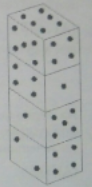
\includegraphics[width=\linewidth]{6K-27}
        \end{figure}
    \end{minipage}
\end{minipage}}
{НаписанноеРешение}
{ВерныйОтвет}{Подсказка}
\end{problem}

\begin{problem}{Задачи на логику.}{9.3.10}{9D}{(лёгкая)}
{В отделе работает 41 человек, из которых каждый знает хотя бы один иностранный язык. Английский знают 22 человека, немецкий~--- 20 человек, французский~--- 19 человек, при этом 8 человек знают английский и французский, 8 человек~--- английский и немецкий и 7~--- французский и немецкий.\\ Сколько человек знает все три языка?}
{НаписанноеРешение}
{ВерныйОтвет}{Подсказка}
\end{problem}

\begin{problem}{Задачи на логику.}{9.3.10}{6K}{(лёгкая)}
{Незнайка выписал семь двузначных чисел в порядке возрастания. Затем одинаковые цифры заменил одинаковыми буквами, а разные – разными. Получилось вот что: ХА, АЙ, АХ, ОЙ, ЭМ, ЭЙ, МУ. Докажи, что Незнайка что-то перепутал.}
{НаписанноеРешение}
{ВерныйОтвет}{Подсказка}
\end{problem}

\begin{problem}{Задачи на логику.}{9.3.10}{6K}{*}
{Вася написал верное утверждение:\\
<<В этой фразе 1/3 цифр~--- цифры 3, а 1/2 всех цифр – цифры 1>>.\smallskip\\
А Коля написал фразу: $\,$
<<В этой фразе 1/... всех цифр~--- цифры $\star$, доли цифр $\star$ и $\star$ одинаковы и равны 1/..., а доля всех остальных цифр составляет 1/...>>.\smallskip\\
Вставь вместо звёздочек три разные цифры, а вместо многоточий~--- три разных числа (или цифры) так, чтобы фраза Коли стала верным утверждением.}
{НаписанноеРешение}
{ВерныйОтвет}{Подсказка}
\end{problem}

\begin{problem}{Задачи на логику.}{9.3.10}{6K}{(лёгкая)}
{Один заколдованный мальчик по средам и четвергам говорит только правду, по понедельникам всегда лжёт, а в остальные дни недели может как соврать, так и сказать правду. Шесть дней подряд его спрашивали, как его зовут, и получили такие ответы: Джон, Боб, Джон, Боб, Пит, Боб. \\Как он ответит на этот вопрос на следующий день?\\
(A) Пит \hfill (B) Боб \hfill (C) Джон \hfill (D) Вася \hfill (E) Нельзя определить.}
{НаписанноеРешение}
{ВерныйОтвет}{Подсказка}
\end{problem}

\begin{problem}{Задачи на логику.}{9.3.10}{6K}{(лёгкая)}
{Шесть человек сидят за круглым столом. По очереди, каждый из них говорит: <<Оба моих соседа, справа и слева~--- лжецы>>. Известно, что лжецы всегда лгут, а остальные говорят правду. Кроме этого, все знают про своих соседей, лжецы ли они. Сколько лжецов за столом?}
{НаписанноеРешение}
{ВерныйОтвет}{Подсказка}
\end{problem}

\begin{problem}{Задачи на логику.}{9.3.10}{6K}{(лёгкая)}
{Шестиногие, семиногие и восьминогие кальмары служат подводному королю. Семиногие кальмары всегда лгут, а остальные всегда говорят правду. Однажды встретились 4 кальмара. Синий кальмар сказал: <<Вместе у нас 28 ног>>, зеленый кальмар сказал: <<Вместе у нас 27 ног>>, жёлтый сказал: <<Вместе у нас 26 ног>>, а красный сказал: <<Вместе у нас 25 ног>>. Какой из кальмаров сказал правду?\smallskip\\
(A) красный\hfill(B) синий\hfill(C) зелёный\hfill(D) жёлтый\\\hspace*{4cm}(E) все кальмары~--- те ещё вруны...}
{НаписанноеРешение}
{ВерныйОтвет}{Подсказка}
\end{problem}

\begin{problem}{Задачи на логику.}{9.3.10}{6K \textcolor{olive}{\textbf{$\spadesuit$}}}{(лёгкая)}
{\vspace{-6mm}\\\begin{minipage}{\linewidth}
    \begin{minipage}{0.5\linewidth}

    Справа изображена головоломка. Задача~--- нарисовать, двигаясь только по сторонам шестиугольников, одну замкнутую петлю (больше никаких отдельных участков и разветвлений быть не должно). Даны некоторые подсказки: цифра внутри шестиугольника показывает, сколько участков петли примыкает к этому шестиугольнику (то есть, сколько сторон из 6 должны быть закрашены).\\ Например, в этом случае в самом-самом \\центре ничего нет, поскольку в центральном шестиугольнике стоит 0.\\
    Нарушать заданные требования (например, у шестиугольника в правом нижнем углу проложить путь не через 2, а через 3 участка) нельзя.

    \end{minipage}
    \hspace{0.05\linewidth}
    \begin{minipage}{0.44\linewidth}
        \begin{figure}[H]
        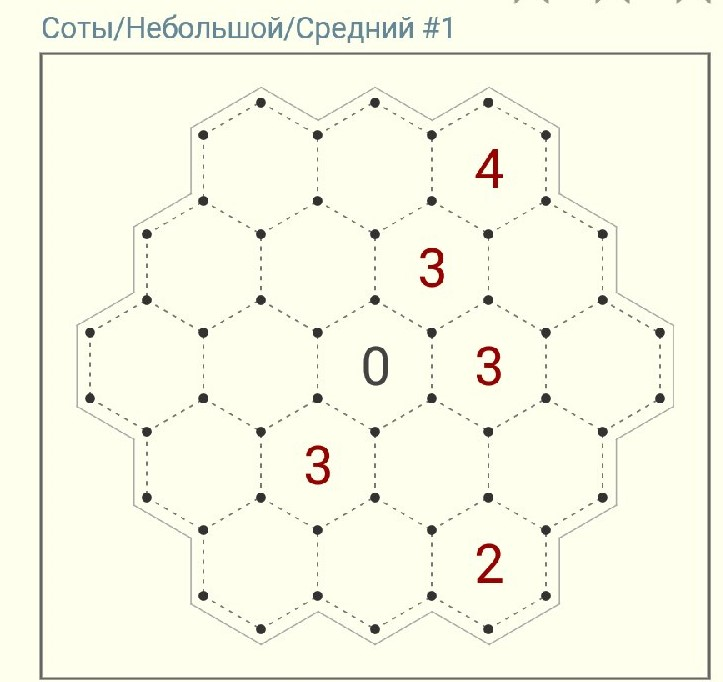
\includegraphics[width=\linewidth]{6K-40}
        \end{figure}
    \end{minipage}
\end{minipage}}
{НаписанноеРешение}
{ВерныйОтвет}{Подсказка}
\end{problem}

\begin{problem}{Задачи на логику.}{9.3.10}{6K \textcolor{olive}{\textbf{$\spadesuit$}}}{(лёгкая)}
{\vspace{-6mm}\\\begin{minipage}{\linewidth}
    \begin{minipage}{0.5\linewidth}

    Справа изображена головоломка. Задача~--- нарисовать, двигаясь только по сторонам шестиугольников, одну замкнутую петлю (больше никаких отдельных участков и разветвлений быть не должно). Даны некоторые подсказки: цифра внутри шестиугольника показывает, сколько участков петли примыкает к этому шестиугольнику (то есть, сколько сторон из 6 должны быть закрашены).\\ Например, в этом случае провести маршрут левее 1 нельзя, поскольку в этом случае участков будет минимум 3, а должен быть ровно один.\\
    Нарушать заданные требования (например, у шестиугольника с цифрой 5 проложить путь только через 4 участка) нельзя.

    \end{minipage}
    \hspace{0.05\linewidth}
    \begin{minipage}{0.44\linewidth}
        \begin{figure}[H]
        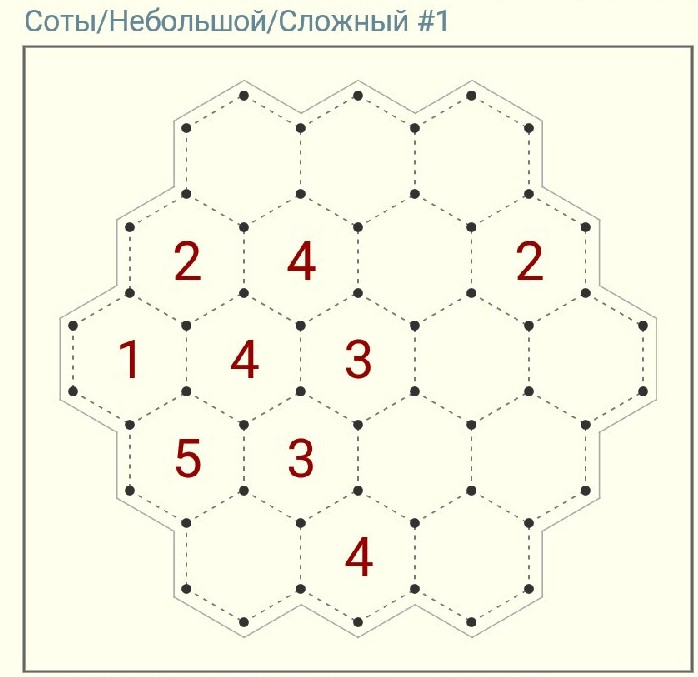
\includegraphics[width=\linewidth]{6K-41}
        \end{figure}
    \end{minipage}
\end{minipage}}
{НаписанноеРешение}
{ВерныйОтвет}{Подсказка}
\end{problem}

\begin{problem}{Задачи на логику.}{9.3.10}{6K \textcolor{olive}{\textbf{$\spadesuit$}}}{(лёгкая)}
{\vspace{-6mm}\\\begin{minipage}{\linewidth}
    \begin{minipage}{0.5\linewidth}

    Справа изображена головоломка.\\ Задача~--- нарисовать, двигаясь только по сторонам четырёхугольников, одну замкнутую петлю (больше никаких отдельных участков и разветвлений быть не должно).\\
    Даны некоторые подсказки: цифра внутри четырёхугольника показывает, сколько участков петли примыкает к этому четырёхугольнику (то есть, сколько сторон из 4 должны быть закрашены).\\
    Нарушать заданные требования, например, рядом с четырёхугольником с цифрой 0 проложить путь через любой участок, нельзя.

    \end{minipage}
    \hspace{0.05\linewidth}
    \begin{minipage}{0.44\linewidth}
        \begin{figure}[H]
        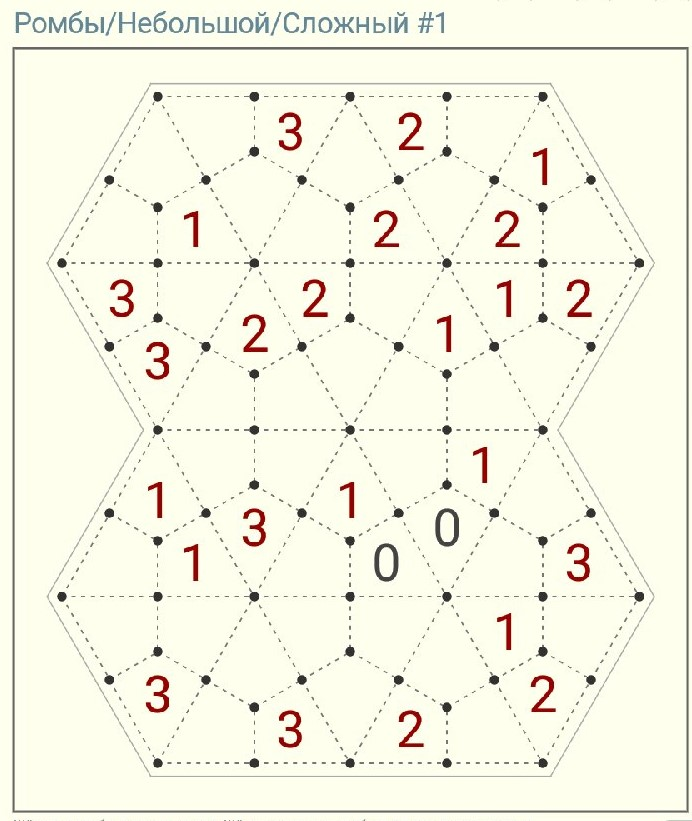
\includegraphics[width=\linewidth]{6K-42}
        \end{figure}
    \end{minipage}
\end{minipage}}
{НаписанноеРешение}
{ВерныйОтвет}{Подсказка}
\end{problem}

\begin{problem}{Задачи на логику.}{9.3.10}{6K \textcolor{olive}{\textbf{$\spadesuit$}}}{(лёгкая)}
{\vspace{-6mm}\\\begin{minipage}{\linewidth}
    \begin{minipage}{0.5\linewidth}

    Эта головоломка больше похожа на судоку. Задача~--- расставить цифры 1, 2, 3, 4 в 16 клеток таблицы справа так, чтобы в каждой строке и каждом столбце эти цифры не повторялись. Также есть некоторые подсказки-ограничения: некоторые клетки объединены вместе арифметической операцией.\\ Например, в правом верхнем углу значок $12\times$ означает, что произведение этих трёх чисел равно 12.\\
    $2-$ означает, что разность двух чисел равна 2,\\ $2\div$ означает, что при делении одного числа на другое получится 2,\\ $5+$ означает, что сумма этих чисел равна 5 (то есть тут это либо 1+4, либо 2+3 в обоих случаях)

    \end{minipage}
    \hspace{0.05\linewidth}
    \begin{minipage}{0.44\linewidth}
        \begin{figure}[H]
        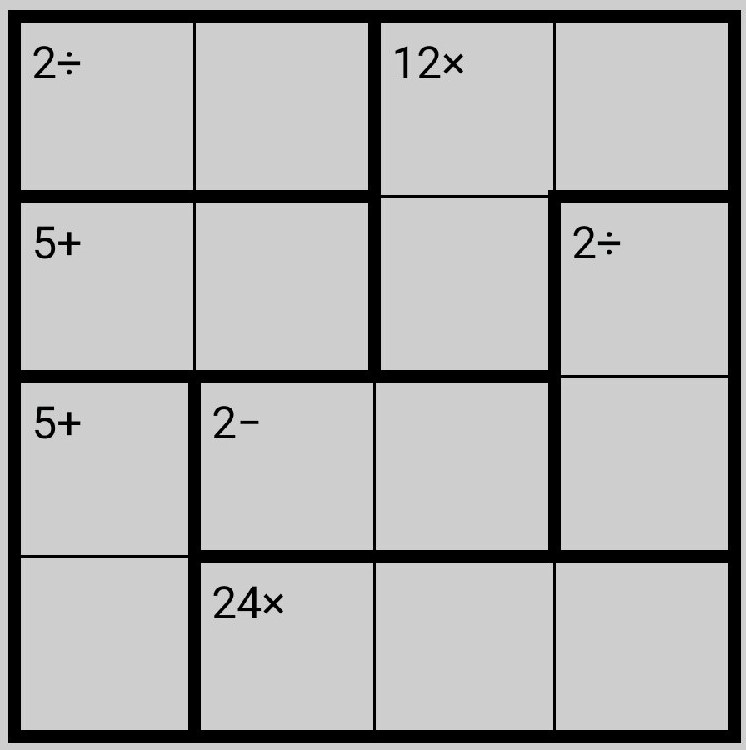
\includegraphics[width=\linewidth]{6K-43}
        \end{figure}
    \end{minipage}
\end{minipage}}
{НаписанноеРешение}
{ВерныйОтвет}{Подсказка}
\end{problem}

\begin{problem}{Задачи на логику.}{9.3.10}{6K \textcolor{olive}{\textbf{$\spadesuit$}}}{(лёгкая)}
{\vspace{-6mm}\\\begin{minipage}{\linewidth}
    \begin{minipage}{0.5\linewidth}

    Головоломка, немного похожая на судоку. Нужно расставить цифры 1, 2, 3, 4 в 16 клеток таблицы справа так, чтобы в каждой строке и каждом столбце эти цифры не повторялись.\\
    В качестве подсказок для некоторых чисел (но не для всех) указано, какие числа больше, а какие меньше: например, число в левом верхнем углу больше, чем то, что стоит в соседней клетке ниже (между ними стоит знак неравенства).

    \end{minipage}
    \hspace{0.05\linewidth}
    \begin{minipage}{0.44\linewidth}
        \begin{figure}[H]
        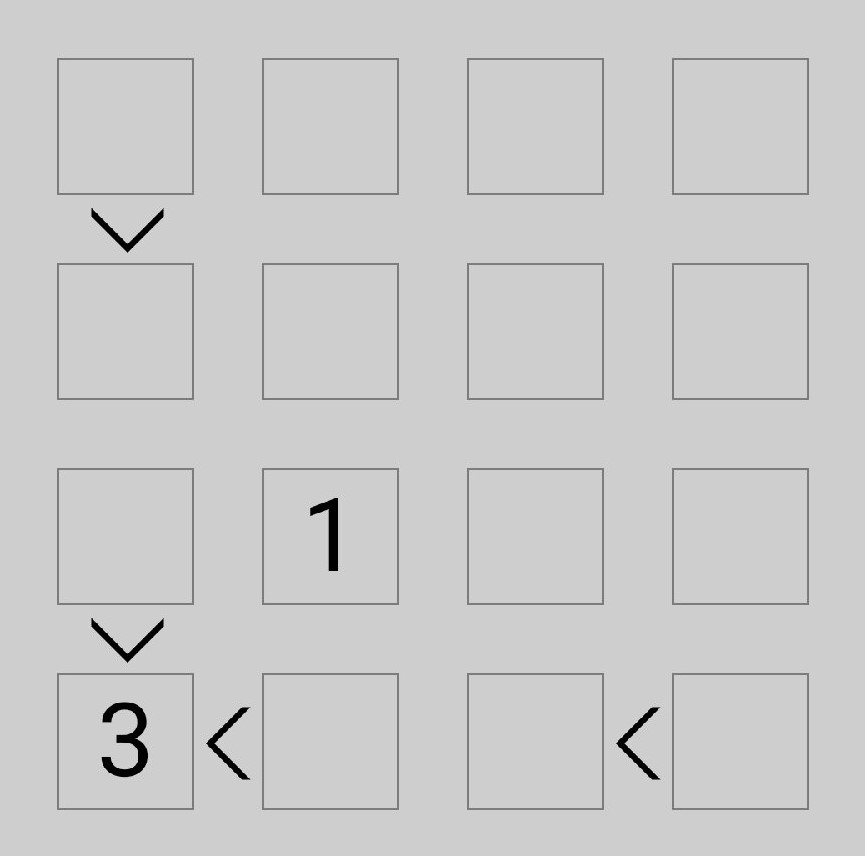
\includegraphics[width=\linewidth]{6K-44}
        \end{figure}
    \end{minipage}
\end{minipage}}
{НаписанноеРешение}
{ВерныйОтвет}{Подсказка}
\end{problem}

\begin{problem}{Задачи на логику.}{9.3.10}{6K \textcolor{olive}{\textbf{$\spadesuit$}}}{(лёгкая)}
{\vspace{-6mm}\\\begin{minipage}{\linewidth}
    \begin{minipage}{0.5\linewidth}

    Головоломка <<Палатки>>.\smallskip\\
    12 групп туристов отправились на отдых, каждая группа со своей палаткой. Они ставят палатки рядом с деревьями (в соседней клетке по горизонтали/вертикали, но не по диагонали), причём две палатки не могут соприкасаться друг с другом даже углами (как корабли в морском бою), а также нельзя ставить палатку к дереву, если у него уже стоит другая палатка.
    Комбинация палатка-дерево-палатка возможна только если одна из палаток <<относится>> к другому соседнему дереву.\\ В качестве подсказки указано общее количество палаток в каждой строке и каждом столбце (цифры справа и снизу от деревьев)~--- например, в первом столбце должно быть 3 палатки.

    \end{minipage}
    \hspace{0.05\linewidth}
    \begin{minipage}{0.44\linewidth}
        \begin{figure}[H]
        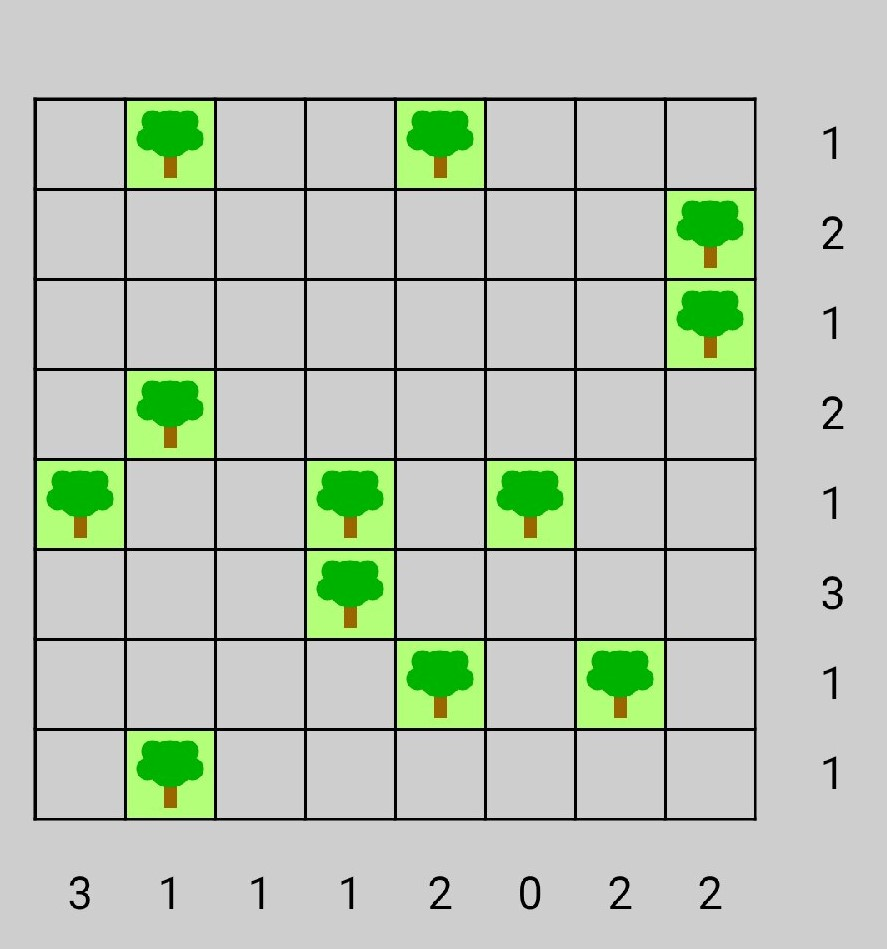
\includegraphics[width=\linewidth]{6K-45}
        \end{figure}
    \end{minipage}
\end{minipage}}
{НаписанноеРешение}
{ВерныйОтвет}{Подсказка}
\end{problem}

\begin{problem}{Задачи на логику.}{9.3.10}{6K}{(лёгкая)}
{В парке растут сосны и дубы. Что может быть верным?
\\(A) Каждый дуб ниже какой-то сосны, и каждая сосна ниже любого дуба;
\\(B) Каждый дуб ниже какой-то сосны, и какая-то сосна ниже любого дуба;
\\(C) Какой-то дуб ниже какой-то сосны, и любая сосна ниже любого дуба;
\\(D) Какой-то дуб ниже любой сосны, и какая-то сосна ниже любого дуба;
\\(E) Все утверждения выше~--- кромешный обман!}
{НаписанноеРешение}
{ВерныйОтвет}{Подсказка}
\end{problem}

\begin{problem}{Задачи на логику.}{9.3.10}{6K}{(лёгкая)}
{В доме $4$ этажа, на которых живут Аня, Боря, Вика, Гена.\\ Известно, что на самом верхнем этаже живёт Аня. Гена живёт выше Бори, и ни один из мальчиков не живёт на чётном этаже. Кто где живёт?}
{НаписанноеРешение}
{ВерныйОтвет}{Подсказка}
\end{problem}

\begin{problem}{Задачи на логику.}{9.3.10}{79I}{(лёгкая)}
{Три подруги вышли на прогулку в туфлях и платьях белого, зелёного и синего цветов. Известно, что только у Ани цвет платья и туфель совпадает; ни туфли, ни платье Вали не белые; Наташа в зелёных туфлях.\\ Определить цвет платья и туфель каждой из подруг.}
{НаписанноеРешение}
{ВерныйОтвет}{Подсказка}
\end{problem}

\begin{problem}{Задачи на логику.}{9.3.10}{79I}{(лёгкая)}
{Есть три коробки, в одной из них чек на круглую сумму, а в двух других~--- пусто. На коробках следующие надписи:\\
1: <<В этой коробке чека нет.>>
\\2: <<В этой коробке лежит чек.>>
\\3: <<Во второй коробке~--- пусто.>>
\\Какую коробку следует выбрать, если известно, что в действительности не более чем одна из этих надписей верна?}
{НаписанноеРешение}
{ВерныйОтвет}{Подсказка}
\end{problem}

\begin{problem}{Задачи на логику.}{9.3.10}{9I}{(лёгкая)}
{Узник выживет, если он пройдёт испытание. Известно, что в одной из комнат сидит принцесса, в другой~--- тигр, а третья комната пуста. При этом надпись на двери комнаты, в которой находится принцесса, истинна, надпись на двери, за которой сидит тигр, ложна, а то, что написано на табличке у пустой комнаты, может оказаться как истинным, так и ложным.
Вот эти таблички:
\\1: <<Комната №3 пуста>>.
\\2: <<Тигр сидит в комнате №1>>.
\\3: <<Эта комната пуста>>.\\
Узник раньше видел принцессу и совсем не прочь жениться на ней.\\ Поэтому, хотя пустая комната, конечно, получше комнаты с тигром, узнику всё же хотелось бы угадать, где принцесса. Так где же принцесса, а где тигр?}
{НаписанноеРешение}
{ВерныйОтвет}{Подсказка}
\end{problem}

\begin{problem}{Задачи на логику.}{9.3.10}{9I}{(лёгкая)}
{Узник выживет, если он пройдёт испытание: нужно угадать, в какой комнате принцесса, а в какой~--- тигр. Неизвестно, сколько в комнатах тигров и принцесс, известно лишь, что комнаты не могут быть пустыми. При этом надпись на двери первой комнаты, если за ней находится принцесса, всегда истинна, а если тигр,~--- ложна, а для второй всё наоборот: надпись истинна, если за второй дверью находится тигр, и ложна, если за ней находится принцесса.\\ Вот эти таблички:\\
1: <<Что ни выберешь, всё едино (либо за обеими дверьми принцессы, либо за обеими дверьми тигры)>>\\
2: <<Принцесса в другой комнате>>.\\
Какую дверь открывать?}
{НаписанноеРешение}
{ВерныйОтвет}{Подсказка}
\end{problem}

\begin{problem}{Задачи на логику.}{9.3.10}{79I}{(лёгкая)}
{Однажды в школе была найдена странная тетрадь.\\ В ней было написано 100 следующих утверждений:\\
<<В этой тетради ровно одно неверное утверждение>>\\
<<В этой тетради ровно два неверных утверждения>>\\
...\\
<<В этой тетради ровно сто неверных утверждений>>.\\
Какие из написанных утверждений верные? (больше в тетради ничего нет)}
{НаписанноеРешение}
{ВерныйОтвет}{Подсказка}
\end{problem}

\begin{problem}{Задачи на логику.}{9.3.10}{6K}{(лёгкая)}
{На время перерыва в классе оставалось девять учеников.\\ Один из них разбил окно.
На вопрос учителя ребята ответили так:\smallskip\\ Аркадий: Это сделал Борис.
\\Василий: Это неправда.
\\Мария: Я его разбила.
\\Егор: Это сделала либо Мария, либо Анна.
\\Борис: Василий лжёт.
\\Тарас: Это была Мария.
\\Леонид: Нет. Мария окно не разбивала.
\\Анна: Ни Мария, ни я этого не делали.
\\Елена: Анна права, но Борис также невиновен.
\\Если мы знаем, что из этих девяти высказываний три, и только три истинны, кто разбил окно?}
{НаписанноеРешение}
{ВерныйОтвет}{Подсказка}
\end{problem}

\begin{problem}{Задачи на логику.}{9.3.10}{6K}{(лёгкая)}
{Стефания вложила некоторую часть своих денег в пять различных компаний: <<Смит и К>>, <<Алако>>, <<Довин Продактс>>, <<Корбетт и сыновья>> и <<Кортелл>>, которые занимаются следующими видами бизнеса: бумажная продукция, алюминий, напитки, краска и обшивка.\\ Суммы ее вложений: 100\$, 200\$, 300\$, 500\$ и 800\$. Недавно Стефания получила информацию о том, сколько денег она заработала или потеряла на каждой из них: 10\% прибыли, 20\% убытков, 30\% прибыли, 5\% убытков и 15\% прибыли.\\ Используя данную ниже информацию, выясните, что продает каждая компания, какую сумму вложила Стефания в каждую из них, её прибыль или потери.\\
1) Компания <<Довин Продактс>> получила 30\% прибыли, доля Стефании составила 30\$.\\
2) Больше всего денег Стефания получила от компании, производящей краски, но это не <<Корбетт и сыновья>> и не <<Кортелл>>.\\
3) Инвестиции в алюминий были большой ошибкой и стоили Стефании 160\$.\\
4) <<Алако>> производит наружную обшивку, а <<Кортелл>> не выпускает прохладительных напитков.\\
5) <<Корбетт и сыновья>> потеряли 20\%.\\
6) Стефания вложила 300\$ в <<Кортелл>>.\\
7) От вложения в 200\$ Стефания потеряла 5\%.\\
8) Компания <<Смит и К>> принесла Стефании прибыль в 50\$.}
{НаписанноеРешение}
{ВерныйОтвет}{Подсказка}
\end{problem}

\begin{problem}{Задачи на логику.}{9.3.10}{79I}{(лёгкая)}
{Пятеро одноклассников: Аня, Саша, Лена, Вася и Миша стали победителями олимпиад школьников по физике, математике, информатике, литературе и географии. Известно, что:
\\1) Победитель олимпиады по информатике учит Аню и Сашу работе на компьютере;
\\2) Лена и Вася после этого тоже заинтересовались информатикой;
\\3) Саша всегда побаивался физики;
\\4) Лена, Саша и победитель олимпиады по литературе занимаются плаванием;
\\5) Саша и Лена поздравили победителя олимпиады по математике;
\\6) Аня сожалеет о том, что у неё остаётся мало времени на литературу.
\\Победителем какой олимпиады стал каждый из этих ребят?}
{НаписанноеРешение}
{ВерныйОтвет}{Подсказка}
\end{problem}

\begin{problem}{Задачи на логику.}{9.3.10}{6K}{*}
{Пятеро подруг~--- Настя, Таня, Света, Галя, Саша~--- решили пойти за покупками в супермаркет. Одна из подруг купила порошок, другая~--- торт, третья~--- книгу, четвёртая~--- музыкальный диск, а пятая~--- сок. Каждая из них израсходовала определенную сумму: одна~--- $70$ рублей, другая~--- $75$ рублей, третья - $80$, четвёртая~--- $100$ и пятая~--- $120$. Фамилии подруг были: Иванова, Ломакина, Казакова, Петрова, Сидорова. Определите имя, фамилию, расходы и покупку для каждой из подруг, если известно, что:
\\1) Настя сок не покупала.
\\2) Подруга, которая купила книгу, заплатила $75$ рублей.
\\3) Казакова потратила $70$ рублей, но не на диск и не на торт.
\\4) Таня Ломакина денег потратила больше, чем Иванова.
\\5) Порошок купила Петрова. Она израсходовала денег больше, чем Галя и Настя.
\\6) $100$ рублей Саша потратила не на торт, а её фамилия не Петрова и не Сидорова.

}
{НаписанноеРешение}
{ВерныйОтвет}{Подсказка}
\end{problem}

\begin{problem}{Задачи на логику.}{9.3.10}{79I}{*}
{Гриша и четыре его соседа учатся в одной школе, но все в разных классах (с 5-го по 9-й). Разумеется, что и классные руководители у них разные (одна из них Вера Борисовна).\\ Кроме того, буквы классов (А, Б, В, Г, Д) ни у кого из них не совпадают.\\ Требуется выяснить, кто в какой класс отправится первого сентября и каковы имена классных руководителей в каждом классе. (Предполагается, что разница в классах равна разнице в возрасте.) Известно, что:\\
1) Ученик <<Г>> класса, Антоша, на два года старше ученика из класса Галины Петровны, a Миша на два года старше ученика из класса Анны Андреевны.\\
2) Один из ребят будет учиться в 8 <<Д>>.\\
3) Ученик из класса <<Б>> на год младше Саши (из класса Марии Ивановны), a Лёша на год младше ученика из класса <<В>> (и это не Миша).\\
4) У Нины Алексеевны <<В>> класс.}
{НаписанноеРешение}
{ВерныйОтвет}{Подсказка}
\end{problem}

\begin{problem}{Задачи на логику.}{9.3.10}{6K}{*}
{Требуется составить рецепты пяти кондитерских изделий (кекс лимонный, коврижка с изюмом, печенье к кофе, торт глазированный, сдобное тесто), в которых присутствуют мука, масло, сахар и яйца.
\smallskip\\1) Муки в различных рецептах требуется: $1$ стакан; $1{,}5$ стакана; $2$ стакана; $2{,}5$ стакана и $4$ стакана.
\\2) Сахара в разные изделия кладут: $1$ ложку; $1/2$ стакана; $3/4$ стакана; $1$ стакан и $1{,}5$ стакана.
\\3) Яйца на кондитерские изделия идут в таких количествах: $1$, $2$, $3$, $4$ и $9$ штук.
\\4) Для коврижки нужно столько муки, сколько для кекса и печенья вместе.
\\5) Зато для кекса нужно вдвое меньше стаканов сахара, чем для торта и печенья вместе взятых.
\\6) А вот для торта нужно столько яиц, сколько для коврижки и сдобного теста, вместе взятых.
\\7) В изделие, требующее двух стаканов муки, идёт $4$ ложки масла; к $3/4$ стакана сахара идёт $2$ ложки масла; к изделию из $2$ яиц кладётся $5$ ложек масла;
\\8) В сдобное тесто надо положить $300$ г масла, а в кекс~--- $3/4$ стакана масла.
\\9) Только в одном рецепте кладут одинаковое количество стаканов муки и сахара.
\\10) На коврижку расходуется более одного яйца, а на сдобное тесто более одного стакана муки.}
{НаписанноеРешение}
{ВерныйОтвет}{Подсказка}
\end{problem}

\begin{problem}{Задачи на логику.}{9.3.10}{79I}{*}
{(Каждому кораблю~--- в свой порт). В порту пять кораблей. Известно, что:
\\1) Греческий корабль отчаливает в $6$. Он везет кофе.
\\2) У корабля, который в середине~--- чёрная труба.
\\3) Английский корабль отплывает в $9$.
\\4) Французский корабль, у которого синяя труба, пришвартован слева от корабля, который везет кофе.
\\5) Справа от корабля, который гружён какао, стоит корабль, который плывёт в Марсель.
\\6) Корабль под бразильским флагом направляется на Манилы.
\\7) Рядом с кораблем, на котором рис~--- корабль с зеленой трубой.
\\8) Корабль, плывущий в Геную, отходит в $5$.
\\9) Испанский корабль отплывает в семь и находится справа от корабля, плывущего в Марсель.
\\10) Корабль с красной трубой направляется в Гамбург.
\\11) Рядом с кораблем, который отчаливает в $7$, корабль с белой трубой.
\\12) На крайнем корабле~--- зерно.
\\13) Корабль с чёрной трубой отплывает в $8$.
\\14) Корабль с зерном пришвартован рядом с кораблем, на котором груз риса.
\\15) Корабль, следующий до Гамбурга, отчаливает в $6$.
\\На каком корабле чай? Куда сесть путешественнику, плывущему в Порт-Саид?}
{НаписанноеРешение}
{ВерныйОтвет}{Подсказка}
\end{problem}

\begin{problem}{Задачи на логику.}{9.3.10}{79I}{*}
{Есть пять человек, разноцветные дома которых расположены в ряд и пронумерованы (слева направо) от №$1$ до №$5$.
У них разные имена, разные профессии и разные пристрастия в еде.
\\$\bullet$ Дома: белый, жёлтый, красный, зеленый, синий.
\\$\bullet$ Имена: Андрей, Василий, Евгений, Николай, Сергей.
\\$\bullet$ Профессии: парикмаxер, пилот, писатель, почтальон, телефонист.
\\$\bullet$ Фрукты-ягоды: ананас, банан, вишня, клубника, персик.
\\$\bullet$ Овощи: баклажан, капуста, перец, томат, тыква.\\
Известно, что:
\\1) Человек в третьем доме любит персики.
\\2) В первом доме живёт Василий.
\\3) Сергей живёт в красном доме.
\\4) Жилец зелёного дома любит ананасы.
\\5) Любитель баклажанов живёт в жёлтом доме.
\\6) Парикмахера зовут Андрей.
\\7) Евгений предпочитает вишни.
\\8) Николай любит капусту.
\\9) Зелёный дом стоит левее белого.
\\10) Писатель предпочитает томаты.
\\11) Любитель клубники из овощей предпочитает перец.
\\12) Белый дом соседствует с зелёным.
\\13) Почтальон живёт рядом с любителем тыкв.
\\14) Соседом пилота является любитель баклажанов.
\\15) Василий живёт рядом с синим домом.
\\16) Соседом любителя бананов является поклонник тыкв.\\
Кто где живёт?}
{НаписанноеРешение}
{ВерныйОтвет}{Подсказка}
\end{problem}

\begin{problem}{Задачи на логику.}{9.3.10}{79I}{*}
{На одной из улиц дачного поселка только 5 домов. Они окрашены в разные цвета, и занимают их семьи поэта, писателя, критика, журналиста и редактора. В доме каждой семьи живёт любимая птичка. Глава семьи получает на завтрак любимый им напиток, после чего отправляется в город, пользуясь любимым способом передвижения. Известно, что:\\
1) Поэт пользуется велосипедом;\\
2) Редактор живёт в красном доме;\\
3) Критик живёт в крайнем доме слева,
а рядом расположен голубой дом;\\
4) Тот, кто ездит на мотоцикле, живёт в среднем доме;\\
5) Тот, кто живёт в зеленом доме, всегда отправляется в город пешком;\\
6) Зеленый дом расположен справа от белого;\\
7) В доме, где живёт снегирь, на завтрак всегда бывает молоко;\\
8) Тот, кто на завтрак получает какао, живёт в доме, соседнем с тем домом, где живёт синица;\\
9) В жёлтом доме на завтрак подают чай;\\
10) Живущий рядом с любителем канареек утром пьет чай;\\
11) Писатель пьет только кофе;\\
12) Тот, кто ездит на своём автомобиле, любит пить томатный сок;\\
13) В доме журналиста живёт попугайчик.\\
У кого живёт сорока? Кто ездит на автобусе?}
{НаписанноеРешение}
{ВерныйОтвет}{Подсказка}
\end{problem}

\begin{problem}{Задачи на логику.}{9.3.10}{79I}{*}
{1) На улице подряд расположены пять домов.
\\2) Англичанин проживает в доме красного цвета.
\\3) Испанец держит собаку.
\\4) В доме зелёного цвета пьют кофе.
\\5) Украинец любит чай.
\\6) Дом зелёного цвета расположен сразу справа от дома белого цвета.
\\7) Курящий <<Old Gold>>, разводит улиток.
\\8) В доме жёлтого цвета живёт курящий <<Kool>>.
\\9) В доме по центру пьют молоко.
\\10) Норвежец живёт в доме №1.
\\11) Сосед курящего <<Chesterfield>> держит в доме лису.
\\12) В доме, соседнем с тем где держат лошадь, живёт курящий <<Kool>>.
\\13) Курящий <<Lucky Strike>> любит апельсиновый сок.
\\14) Японец курит <<Parlament>>.
\\15) Норвежец живёт в доме, расположенном рядом с домом синего цвета.\\
Вопрос: Кто пьёт воду, а кто держит зебру?}
{НаписанноеРешение}
{ВерныйОтвет}{Подсказка}
\end{problem}

\begin{problem}{Задачи на логику.}{9.3.10}{9D}{*}
{Для прохождения теста тысячу мудрецов выстраивают в колонну. Из колпаков с номерами от 1 до 1001 один прячут, а остальные в случайном порядке надевают на мудрецов. Каждый видит только номера на колпаках всех впереди стоящих. Далее мудрецы по порядку от заднего к переднему называют вслух целые числа. Каждое число должно быть от 1 до 1001, причём нельзя называть то, что уже было сказано. Результат теста~--- число мудрецов, назвавших номер своего колпака. Мудрецы заранее знали условия теста и могли договориться, как действовать (придумать любую стратегию)
\\a) Могут ли мудрецы гарантировать результат более 500?
\\b) Могут ли мудрецы гарантировать результат не менее 999?}
{НаписанноеРешение}
{ВерныйОтвет}{Подсказка}
\end{problem}

\begin{problem}{Задачи на логику.}{9.3.10}{79I}{*}
{На одной улице (в неизвестной последовательности) стоят в одну линию 6 домов:\\ красный, синий, жёлтый, зеленый, белый и коричневый. Имена жителей: Алекс, Боря, Вова, Гоша, Дима и Егор. Места их работ: МВД, ФСБ, КГБ, ЦРУ, ФБР, и 911. У каждого из них только один, отличный от других автомобиль: BMW, VOLVO, FIAT, FORD, AUDI и ГАЗ. В каждом доме есть компьютер, но с разными процессорами: i486, MMX, PII, P3, AMD и CYRIX. Любимым лакомством каждого являются или только яблоко, или груша, или апельсин, или банан, или вишня, или клубника.\\ Кроме этого известно, что:\\
1) Тот, кто работает в МВД, живёт в красном доме.\\
2) В коричневом доме живёт Алекс и у него AMD.\\
3) Владелец машины марки FORD обожает апельсины.\\
4) Владелец PII имеет автомобиль ГАЗ.\\
5) У Гоши дома компьютер с процессором MMX.\\
6) Владелец AUDI имеет CYRIX, работает на ФБР и живёт в жёлтом доме.\\
7) Служащий в КГБ работает на i486.\\
8) FIAT ставится в гараж по соседству с зеленым домом.\\
9) Егор живёт по соседству с ЦРУшником.\\
10) Боря живёт рядом с тем, у кого PII.\\
11) Владелец VOLVO живёт рядом с любителем клубники.\\
12) Вова живёт рядом с любителем груш.\\
13) Служака из МВД~--- сосед любителя вишни.\\
14) У работника ФСБ по соседству находится CYRIX.\\
15) Любители груш и яблок живут рядом.\\
16) Синий дом стоит с краю.\\\
17) Рядом с белым домом живёт работник службы 911.\\
18) В соседних домах находятся P3 и FIAT.\\
19) В соседних домах паркуются ГАЗ и BMW.\\
20) Дима живёт по соседству с коричневым домом.\\
21) У владельца AMD по соседству жёлтый дом.\\
22) Красный дом находится правее коричневого.\\
23) Через дом от Гоши живёт КГБшник, а между ними~--- работник МВД.\\
24) Через дом от Димы живёт ЦРУшник, и между ними нет компьютера с CYRIX.\\
Определить последовательность домов, имена проживающих в них, а так же их места работы, марки автомобилей, тип процессора и любимое лакомство.}
{НаписанноеРешение}
{ВерныйОтвет}{Подсказка}
\end{problem}

\end{document}